% 
%% Replace 'XX' with your paper number (assigned when you register abstract)
%% Replace 'NN' with actual number of pages. 

\documentclass[letterpaper,twocolumn,10pt]{article}
\usepackage{usenix2019,epsfig,subcaption}
%========================
%  Packages
%========================
%\usepackage{datetime}
\usepackage{url}
%\usepackage{hyperref}
\usepackage{color}
%\usepackage{graphicx}
\usepackage{algorithm}
\usepackage[noend]{algpseudocode}

%========================
%  Macros
%========================

\newcommand{\code}[1]{\textsf{\fontsize{9}{11}\selectfont #1}}

\newcommand{\inred}[1]{{\color{red}{#1}}}
\newcommand{\remove}[1]{}
\newcommand{\Idit}[1]{\inred{[Idit: #1]}}

\newcommand{\sys}{YoDB}

\newcommand{\tuple}[1]{\ensuremath{\langle \mbox{#1} \rangle}}

\usepackage{cleveref}


\crefformat{section}{\S#2#1#3}




% No date in title area
\date{}


% Actual document begins below.
\begin{document}

\title{\Large \bf \sys: Rethinking Design Principles for Key-Value Storage} 
\author{}
\maketitle

\subsection*{Abstract}
Many applications of key-value (KV-)storage exhibit high \emph{spatial locality}
of access, for example, when data items with identical composite key prefixes are created and  scanned together.  
This prevalent access pattern is underused by the ubiquitous LSM tree design underlying KV-stores today.
%
We present \sys, a persistent KV-store targeting spatially-local workloads. \sys\ forgoes the temporal data organization 
of LSM trees, and partitions data by key, both in memory and on disk. 
In workloads with high locality, \sys\  consistently outperforms the state-of-the-art. 
For example, its range scan throughput in workloads with composite keys is \inred{1.25x to 3x} higher than that 
of RocksDB -- an industry-leading LSM database.  \sys\/ further reduces write amplification 
by up to \inred{2.6x}, thereby contributing to slower device wear. \sys\/ scales on multicore platforms and provides strong (atomic) guarantees for updates, lookups, and scans. 
%Finally, it provides consistent crash recovery semantics, with near-instant recovery time. 

\section{Introduction}
%%%%%%%%%%%%%%%%%%%%%%%%%%%%%%%%%%%%%%%%%%%%%%%%%%%%%%%%%%%%%%%%%%%%%%%%%
\subsection{Motivation:  spatial locality in KV-storage}
% KV-storage workloads} 
%%%%%%%%%%%%%%%%%%%%%%%%%%%%%%%%%%%%%%%%%%%%%%%%%%%%%%%%%%%%%%%%%%%%%%%%%

% KV-stores are everywhere
Key-value stores (KV-stores) are widely used  by a broad range of applications and are projected
to continue to increase in popularity in years to come; market research  identifies them as the 
``driving factors'' of the NoSQL market, which is expected to garner \$4.2B by 2020~\cite{alliedmarketresearch}.

% In many applications, keys are composite
KV-stores provide a simple programming model. 
Data is an ordered collection of key-value pairs, and the API supports random writes, 
random reads, and range queries. 

A common design pattern is the use of \emph{composite} keys that represent an agglomerate of attributes.
Typically, the primary attribute (key prefix) %-- called the \emph{primary key} -- 
has a skewed distribution, and so   access via the composite key exhibits \emph{spatial locality}, as 
popular key prefixes result in popular key ranges~\cite{facebook-workloads}. 

One example of this arises in mobile analytics platforms, e.g., AppsFlyer~\cite{appsflyer}, Flurry~\cite{flurry}, 
and Google Firebase~\cite{firebase}. %~\cite{medium-mobile-analytics}.   
Such platforms %help mobile developers collect user activity data, analyze it, and optimize their app experience. They 
ingest massive streams of app event reports %(e.g., start, stop, or particular scenario within an app), 
in  real-time and provide a variety of insight queries into the data. For example, Flurry tracked events from  
1M+ apps across 2.6B user devices  in 2017~\cite{FlurryReport2017}. In order to offer per-app analytics efficiently,
such services aggregate data in KV-stores indexed by a composite key prefixed by a unique app 
id,  followed by a variety of other attributes (time, user id, device model, location, event type, etc.).
%
We examine a trace of almost $2$B  events captured from a production mobile analytics engine 
over half an hour.  
\Cref{fig:cdf} shows the access frequency distribution over the  $60$K app ids occurring in this stream. It follows a marked
heavy-tail pattern: 
%$10$\% of the apps cover over $99.5$\% of the events; 
$1$\% of the apps  cover $94$\% of the events, and fewer 
than $0.1$\% cover $70$\% of them. 

% This means the data is highly skewed and with a very long tail (not depicted in the figure).
%Table~\ref {table:popular} shows the cumulative probability of the top-$20$ popular applications, covering more than $50$\% of the events. 
%With application name as the primary dimension of a composite key this distribution induces high spatial locality.


\begin{figure}[tb]
\centering
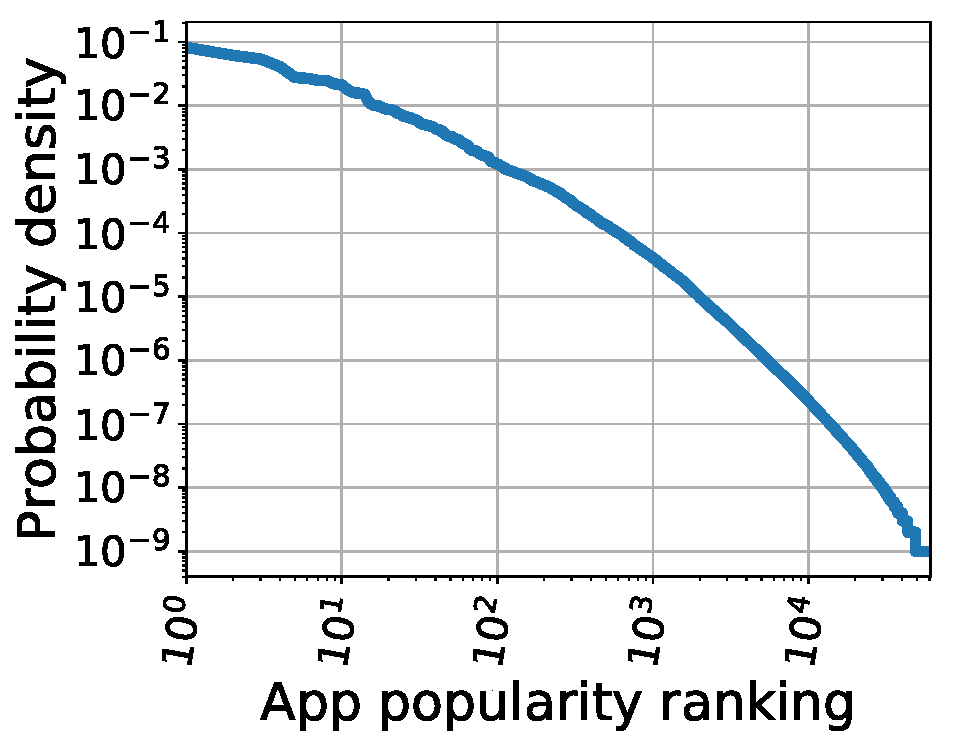
\includegraphics[width=0.6\columnwidth]{figs/app_names_loglog_line.pdf}
\caption{{Distribution of mobile app events by app id (log-log scale) in a production analytics feed (2B events).}}
\label{fig:cdf}
\end{figure}

Composite keys arise in many additional domains, including messaging and social networks~\cite{facebook-workloads}. 
For example, a backend Facebook Messenger query may retrieve the last 100 messages for a 
given user~\cite{Borthakur:2011:AHG:1989323.1989438}; %, where the primary key is user id. 
in Facebook's social network, a graph edge is indexed by a key consisting of two 
object ids and an association type~\cite{Armstrong:2013:LDB:2463676.2465296}.
%Note further that 
Spatial locality   also arises with simple (non-composite) keys, for example, when 
reverse  URL domains are used as keys for web  indexing~\cite{Cho:1998:ECT:297805.297835}. 

% Overfitting for Zipf 
The prevalence of skewed (e.g., Zipfian)  access  in real workloads is widely-recognized 
and reflected in standard benchmarks (e.g., YCSB~\cite{YCSB}). %  feature heavy-tailed key-access distributions like Zipf.
But these benchmarks fail to capture the spatial aspect of locality, which has gotten far less attention.
% Idit: removed below, too bold
%This, in turn, leads to storage systems being optimized for a skewed distribution on individual keys, % with no spatial locality,
%e.g., in partitioning data by  recent access time as opposed to by key range.
In this work, we make spatial locality a first-class consideration in KV-store design.
% which leads us to rethink the design principles underlying today's popular KV-stores.



%%%%%%%%%%%%%%%%%%%%%%%%%%%%%%%%%%%%%%%%%%%%%%%%%%%%%%%%%%%%%%%%%%%%%%%%%
\subsection{Spatial locality: the challenge}  
\label{ssec:B-tree-compare}
%%%%%%%%%%%%%%%%%%%%%%%%%%%%%%%%%%%%%%%%%%%%%%%%%%%%%%%%%%%%%%%%%%%%%%%%%



% LSM is the standard 
The de facto standard design for high-throughput KV-stores today is \emph{LSM} (log-structured merge) trees~\cite{DBLP:journals/acta/ONeilCGO96}. 
LSMs initially group writes  into files \emph{temporally} rather than by key-range. 
A background \emph{compaction} process later merge-sorts any number of files, grouping data by keys. 

% LSM is  not ideal for spatial locality  because of  temporal grouping 
This approach is not ideal for workloads with high spatial locality for two reasons. 
First,  popular key ranges are fragmented across many files. 
Second,  compaction  is costly in terms of  both performance 
(disk bandwidth) and \emph{write amplification}, namely the number of physical writes 
associated with a single application write. The latter is  particularly important in SSDs as it increases disk wear. 
The temporal grouping means that compaction is indiscriminate with respect to key popularity:  
Since new  files are always merged with old ones, 
 ``cold'' key ranges  continue to be repeatedly re-located by  compactions.  

% LSM is not the best when the entire working set fits in memory
Another shortcoming of LSM is that its temporal organization, while optimizing disk I/O,  penalizes in-memory operation. 
All updates -- including ones of popular keys -- are flushed to disk, even though persistence is assured via a separate \emph{write-ahead-log (WAL)}.
%Beyond increasing write amplification, this makes the flushed keys unavailable for fast read from memory,
%which is  wasteful if the system incorporates sufficient DRAM to hold most of the active working set. 
%The drop in DRAM prices (more than $6.6\times$ since 2010~\cite{dram-prices}) makes the latter scenario increasingly common.  

Yet  LSMs have supplanted the  traditional spatial data partitioning of B-trees for a reason~\cite{rocks-vs-inno}.
%A crucial challenge arising in spatially-organized  storage is how to persist all updates in a consistent way without sacrificing performance.
In  B-trees, each update induces random I/O  to a leaf, resulting in poor write performance.
Moreover, the need to preserve a consistent image of a leaf while it is being over-written induces high write amplification. 
$B^{\epsilon}$-trees~\cite{Brodal:2003:LBE:644108.644201} mitigate this cost using write buffers. % in internal tree nodes. 
However, this slows down lookups, which now have to search in unordered buffers, possibly on disk. 
% If the buffers reside on disk, the lookup time is unacceptably slow, whereas if they are in RAM then they have to be complemented by a separate persistence mechanism, with its own costs.  
%
LSMs, in contrast, achieve high write throughput by absorbing  writes in memory and periodically flushing them as 
sequential files to disk; they expedite reads by caching data in DRAM.

The resounding performance advantage of the LSM approach over B- and B$^{\epsilon}$-trees has been repeatedly demonstrated, 
e.g., in a recent  study of the Percona MySQL server using three storage engines -- RocksDB, TokuDB, and InnoDB --
based on LSM, a B$^{\epsilon}$-tree, and a B-tree, respectively~\cite{toku-rocks-inno}.
%
Another advantage of LSMs is that they readily ensure consistency under multi-threaded access -- in particular, atomic scans --   
via lock-free multi-versioning.
%This can be  tricky when a scan spans both memory-resident and disk-resident data.
In contrast, databases based on B- or  B$^\epsilon$-trees either use locks~\cite{innodblocking} 
or forgo scan consistency~\cite{tucana}.



\remove{
Obviously, we do not claim that spatial data partitioning is new; indeed, classical B-trees~\cite{DBLP:conf/sigmod/BayerM70,Comer79} 
 pre-date  LSM trees, and many B-tree variants~\cite{Brodal:2003:LBE:644108.644201,Bender15, Lehman:1981:ELC:319628.319663} have  emerged over the years. 
 However, it is important to note that these trees are  conceptual constructs rather than storage systems; 
 employing these concepts within a practical data store over a memory hierarchy 
 raises multiple challenges,  which perhaps explains their limited adoption in industrial KV-stores.
 A key challenge is what to persist when and in what format. 
 }
 
Our  goal is to 
%draw attention to the importance of spatial locality in today's KV-store workloads and to 
put forth a KV-store design alternative  suited for the 
spatial locality arising in today's  workloads, without forfeiting the benefits achieved by the LSM approach.




%%%%%%%%%%%%%%%%%%%%%%%%%%%%%%%%%%%%%%%%%%%%%%%%%%%%%%%%%%%%%%%%%%%%%%%%%
\subsection{Our contribution: \sys}
%%%%%%%%%%%%%%%%%%%%%%%%%%%%%%%%%%%%%%%%%%%%%%%%%%%%%%%%%%%%%%%%%%%%%%%%%

% Drum roll 
We present \sys, a high-throughput persistent KV-store geared towards spatial locality. 
\sys's  architecture (\cref{sec:principles}) combines a spatial data organization with LSM-like  batch I/O. 
The pillars of our design are large \emph{chunks} holding contiguous key ranges. 
\sys's chunks are not merely  a means to organize data on-disk (like nodes in a B-tree). They 
are also the basic units for read-write DRAM caching, I/O-batching, logging, and compaction. 
This approach is unique.
%Typical KV-stores rely on OS-managed page caches (whereas chunks consist of many pages)  
%supplemented by application-level caches. 
Typical KV-stores rely on finer-grain OS- and application-level page caches (whereas chunks consist of many pages) and employ a global WAL. 

\remove{
B-trees, e.g., InnoDB, use read-write page caches~\cite{InnoDB-Buffer-Pool}, however they fail to capture spatial locality 
because their cache granularity is too fine, which results in poor-performing near-random writes~\cite{toku-rocks-inno}.  
LSM's, e.g., RocksDB, use caches for the read path only~\cite{RocksDB-blockcache}. Their temporal structure optimizes write
performance in the short term but degrades it in the long term, due to compactions. Here too, 
spatial locality remains unexploited.}

Our novel chunk-based organization has several benefits. 
First, chunk caching is effective for spatially-local workloads.
Second, chunk-level logging eliminates the need to log each update in a system-level WAL, thus 
reducing write amplification and expediting crash-recovery. 
Finally, using the same data structure for both the read-path (as a cache) and the write-path
(as a log) allows us to perform \emph{in-memory compaction}, reducing write amplification even further.

% Downsides
The downside of spatial partitioning is that if the data lacks spatial locality and the active working set is big, 
chunk-level I/O batching is ineffective. Moreover, 
caching an entire chunk for a single popular key is wasteful. 
We mitigate the latter by adding a \emph{row cache} for read access to hot keys. Even so, 
our design is less optimal for mixed read/write workloads lacking spatial locality, for which the LSM approach may yield better performance.  

%To further expedite access in different scenarios, we incorporate a number of additional mechanisms: 
%a volatile index for direct access to chunks by key; Bloom filters to reduce reads from disk-resident chunks; and 

Our algorithm (\cref{sec:design}) is designed for high concurrency. 
%among threads running put, get, and scan operations, as well as background maintenance (compaction). 
It supports atomic scans using low-overhead multi-versioning, where versions are increased only by scans and not by updates. 
It ensures consistency and correct failure-recovery. 
%While the mechanisms we employ are all variants of ones appearing in the literature, their combination is novel and results in a high-performance storage system.

We implement \sys\ in  C++ (\cref{sec:impl}) and extensively evaluate it (\cref{sec:eval})
via three types of workloads: (1) a production trace collected from a large-scale mobile analytics platform; 
(2)  workloads with synthetically-generated composite keys exercising  standard YCSB scenarios~\cite{YCSB};
and (3)  YCSB's traditional benchmarks, which employ simple (non-composite) keys.  
%In all cases, 
We compare \sys\ to the recent (Oct 2018) release of RocksDB~\cite{RocksDB}, a mature industry-leading LSM KV-store. 
We  experimented with two additional open-source KV-stores, PebblesDB~\cite{PebblesDB}  and  
% PreconaFT/
TokuDB~\cite{TokuDB} (the only publicly-available $B^{\epsilon}$-tree-based 
KV-store); both performed significantly worse than  RocksDB and \sys, so we focus on RocksDB results. 
%so we do not discuss them further.
%\inred{across the entire YCSB benchmark suite.} %, which is in line with previous studies of PerconaFT~\cite{tucana}, so we excluded them from further tests. 
Our main findings are: 
\begin{enumerate} 
  %   \setlength{\itemindent}{-10pt}
\item \sys\/ is  better than RocksDB under high spatial  locality.  
For instance, on a 256GB production dataset, \sys\ ingests data $4.4\times$ faster than RocksDB %,  scans recent  data up to 27\% faster, 
and reduces write amplification by almost $4\times$. 
%And in large synthetic composite-key workloads, \sys\  improves over RocksDB's throughput by $24\% - 75\%$. 
\item \sys\/ significantly outperforms RocksDB whenever most of the working set fits in RAM, 
%For example, with synthetic composite keys and a memory-resident working set, \sys\  
accelerating scans by up to $3.5\times$, puts by up to $2.3\times$, and gets by up to $2\times$. 
\item \sys's performance is  comparable to RocksDB's in traditional YCSB workloads without spatial locality.
%while its write amplification is much smaller.
\item RocksDB outperforms \sys\ (by 20--25\%)  in mixed read/write workloads with large active working sets and no spatial locality, 
although \sys's write amplification remains $\sim2\times$ smaller than RocksDB's. 
%\item \sys\ has lower write amplification, especially on large datasets.
\end{enumerate}

% Benefits
Our results underscore the advantages of \sys's spatially-organized chunks:
(1) eliminating fragmentation of key ranges  yields better  performance under spatial locality; 
(2) keeping hot ranges in memory leads to better performance when most of the working set fits in RAM; and 
(3) in-memory chunk compaction saves disk flushes and reduces write volume.  
In addition, in-chunk logging allows quick recovery from crashes with no need to replay a WAL.


~\cref{sec:related}  surveys related work and~\cref{sec:conclusions} concludes this paper. 


\section{Design Principles}
\label{sec:principles}


\sys\ is a persistent key-value store supporting atomic \emph{put, get}, and  \emph{range scan} (or scan) operations. 
Scans are atomic in the sense that all values returned by a single scan belong to a consistent snapshot reflecting
the state of the data store at a unique point in time.

\remove{
\sys\ is geared for high-throughput analytics applications, which (1) perform many range scans; 
(2) strive to accommodate the entire working set in RAM (for performance), and yet require  (3)
persistence with fast recovery. 

We now detail the key requirements from \sys\ and the design choices we made in order to meet them.

\subsection{Requirements}

The key requirements from \sys\ are  the following:
}

Our Key design goals are the following:
\begin{enumerate}\itemsep0pt
\item \emph{Optimizing for spatial locality and atomic scans.}
 Many applications support multi-dimensional exploration of data, 
 which they realize in a KV-store using composite keys. This induce spatial locality.  
 \remove{For example, a typical  KV-map used by an application like Flurry Analytics~\cite{flurry} 
 summarizes mobile traffic statistics grouped by a combination of dimensions like  date,  user-id, and application-id.}
In addition, a query that retrieves data pertaining to a particular dimension thus needs to atomically 
retrieve the values pertaining to a range of keys. 
%To favor analytics queries, it is important to optimize such scans. 
 

\item \emph{High performance and low write amplification with memory-resident working sets.}
To sustain high throughput, key-value stores nowadays leverage increasing DRAM sizes where they can hold most of the 
active data set. We strive for maximum performance in this ``high performance'' case.  
In addition to performance, we seek to minimize disk writes in order to reduce disk wear.

\item \emph{Fast recovery.}
Because crashes are inevitable, the mean-time-to-recover from crashes should be kept short.
Like other popular KV-stores~\cite{RocksDB,leveldb,hbase}, \sys\ supports \emph{asynchronous} persistence, 
where put requests are buffered in memory and periodically persisted to disk in bulk. 
This approach significantly reduces the latency of put operations, which do not wait for their data to be persisted.
The downside of this approach is potential loss of recently written data upon crash. 
\remove{For example, 
if data is flushed to disk every $10$ seconds, then put operations executed in the last $10$ seconds before the crash 
may be undone. 

Nevertheless, \sys\ ensures 
}
It is required that \emph{data consistency} is preserved following recovery, in the sense that 
if some put is lost, all ensuing (and thus possibly dependent) puts are lost as well, and the recovery is to a well 
defined execution point some time before the crash.
 
\remove{
 \paragraph{Low write amplification.} 
 Minimizing disk writes is important not only for performance, but also for disk wear reduction.
}
\end{enumerate}

%\subsection{Design choices}

Given the aforementioned requirements, we make the following design choices in \sys:

\begin{enumerate}\itemsep0pt
\item \emph{Chunk-based organization.}
We organize data, both on-disk and in-memory,  in large chunks pertaining to  key ranges.  
%This enables efficient support of range scans, with  high cache locality and minimal loading of new memory pages. 
%Both the read and the write path go through chunks. 
Each chunk has a file representation called  \emph{funk} (file chunk), and may be cached in a  memory data structure called \emph{munk} (memory chunck).
This organization exploits spatial locality and is friendly to range scans.

We use a number of techniques to optimize in-memory  access, including partially sorting keys in each chunk and 
indexing munks. 
To expedite access to  keys whose chunks are only on-disk  (i.e., have no munks), 
individual popular keys are cached in a \emph{row cache}, 
and \emph{Bloom filters} are used to limit excessive access to disk. 

\item \emph{Infrequent disk compactions.}
As long as a chunk is cached (has a munk), its funk's organization does not have to be optimized since 
queries do not access it. Therefore, \sys\ infrequently performs reorganization (compaction) on such funks.
Conversely, when a funk holds cold data, its organization hardly deteriorates, and therefore compaction is not necessary.
Note that this is unlike LSM-trees, where all disk components are compacted, regardless of which keys reside in memory and whether 
keys are hot or cold. 

\item \emph{Multi-versioning for atomic scans.}
\sys\ employs multi-versioning along with
copy-on-write to keep data versions required by atomic scans. 
In other words, if a put attempts to overwrite a key  required by an active scan, then a new version is created alongside the 
existing one, whereas versions that are not needed by any scan are not retained. 
Thus, version management incurs a low overhead (as it occurs only on scans). 
%It also defines a simple rule for garbage collecting old versions.

\item \emph{In-funk WALs.}
\sys\ logs writes within funks and refrains from duplicating the updates  in a separate WAL. This reduces write amplification and expedites recovery times. 
\end{enumerate}


\section{\sys's Design}
\label{sec:design}


The API of \sys\ is presented in Section~\ref{ssec:api}. 
Section~\ref{ssec:layout} then discusses \sys's data organization. 
%Detailed description of \sys's operations is given in Section~\ref{ssec:ops}.  
Atomic scans are discussed in Section~\ref{ssec:scans}, and 
the data structure's maintenance is discussed in Section~\ref{ssec:rebalance}.

\subsection{API and guarantees}
\label{ssec:api}

\sys\ is a persistent key-value store supporting \emph{put, get}, and atomic \emph{range scan} (or scan) operations. 
Scans are atomic in the sense that all values returned by a single scan belong to a consistent snapshot reflecting
the state of the data store at a unique point in time.

\Idit{More on API?}

\sys\ ensures \emph{durability} of all updates by writing updates to disk synchronously as part of the \emph{put} operation.

\subsection{Data organization}
\label{ssec:layout}

\begin{figure}[htb]
\centerline{
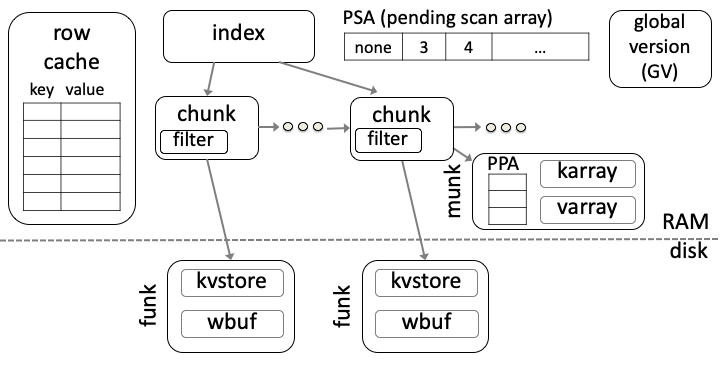
\includegraphics[width=0.9\columnwidth]{PiWi.png}
}
\caption{\sys\ data layout.}
\label{fig:layout}
\end{figure}

\paragraph{Chunk-based layout.}

\sys's data layout is depicted in Figure~\ref{fig:layout}.
Similarly to BTrees \Idit{and other disk-friendly data structures?}, 
\sys\ organizes data in fixed-size \emph{chunks}, each holding a contiguous key range.
This improves the efficiency of both disk access and memory access, in particular, for large range scans. 
At run-time, a list of all chunks is kept in RAM, where each chunk's data 
(consisting of keys in the corresponding range and values associated with them) 
is kept on disk (for persistence), and possibly in memory (for fast access). 

On disk, each chunk is associated with a \emph{file chunk}, or \emph{funk} --
a persistent data structure consisting of three files:  a value store \emph{vstore}, 
a compacted and sorted  key store \emph{kstore}, and a write buffer \emph{wbuf}. The vstore holds all the values associated with keys
in the chunk. When a funk is created, the kstore holds all the chunk's keys with pointers to corresponding values and the wbuf is empty.
New keys are subsequently appended to the unsorted wbuf, while new values are appended to the chunk's vstore.

This structure allows us to benefit from sorted searches on the kstore, and at the same time
allows for updating chunks without re-writing existing data, thus minimizing write amplification.
As a funk's wbuf grows, however, searching becomes inefficient   and  
the funk is no longer compact, i.e., it may contain redundant (over-written keys).
Therefore, once the wbuf exceeds a certain threshold, we reorganize the funk.

Since updates to disk are executed synchronously,  the data store reflecting all completed put operations 
can be consistently recovered from the on-disk funks at any time. \Idit{Need to discuss recovery somewhere.}

A subset of the chunks is also cached in memory to allow fast access, where each cached chunk is associated with a
\emph{memory chunk (munk)}  data structure. 
Munks are volatile and can be removed and recreated from funks at any time.
Thus, multiple \emph{generations} of munks may exist for a chunk throughout its life time.


At run-time, \sys\ holds in memory a linked list of chunk objects as well as 
%representing all funks in the data store. Chunks are also indexed in-memory for fast access by key using 
a \emph{chunk index}, which is a sorted map from keys to chunks (e.g., a sorted array, skip list, or search tree).
Note that since chunk objects do not hold actual keys and values, they are significantly smaller than munks and funks. 
\inred{A typical chunk object is smaller than 1KB, whereas the size of a funk or munk that holds 10K to 100K keys 
ranges between 1M to 100M depending on the data size. A typical \sys\ node holds thousands of chunks, with 
all chunk objects in memory in addition to hundreds of munks.} 


A munk consists of two arrays -- karray and varray -- where the karray implements a sorted linked list of the chunk's keys. 
When a munk is created, its karray is sorted by key, so each cell's successor in the linked list is the ensuing cell in the array.
As new keys are added, they create bypasses in the linked list and karray is no longer sorted.
Key removals, in turn, leave obsolete values in the karrray, so it is no longer compacted.

As key-value pairs are added, overwritten, and removed, munks and funks need to undergo reorganization. This includes  
\emph{compaction} to deallocate removed and overwritten data, 
\emph{sorting} keys to make searches more efficient,  and
\emph{splitting} overflowing chunks.
\remove{, and \emph{merging} under-utilized ones.}
All reorganizations are performed by \sys's \emph{rebalance} operation.
If the chunk has a munk, then rebalance compacts and sorts the munk in-memory by creating a new 
(compacted and sorted) munk instead of the existing one. 
Funks of uncached chunks are also compacted by replacing them with new funks, albeit less frequently.
Splits  create new chunks as well as new  funks (and possibly munks) associated with them.


\paragraph{Data structures.}

In addition to the chunk list and chunk index, \sys\ keeps a \emph{global version (GV)} for supporting atomic snapshot scans,
as described below; it tracks active scans in a \emph{pending scan array (PSA)} for garbage collection purposes (old 
versions not needed by any active scan can be reclaimed).

The chunk data structure is given in Algorithm~\ref{alg:chunk}. 
The first field is its status, which is explained  below. 
It next holds a pointer to the appropriate funk, and, if applicable, also munk, as well as a pointer to the next 
chunk in the chunk linked list.
It further keeps the generation number of its latest munk and a per-generation sequence number,
which, in case there is an active munk, is the index of the next free cell in the munk's karray and varray.


\begin{algorithm}[htb]
\begin{algorithmic}
\State status \Comment  baby, child, active, asleep, or aged
\State ptr funk \Comment funk disk address
\State ptr munk \Comment munk memory pointer
\State ptr next \Comment next chunk in linked list
\State int gen \Comment munk generation
\State int seq \Comment sequence number in current generation 
\State asymmetric lock rebalanceLock \Comment r/w lock 
\State lock funkChangeLock \Comment acquired with try\_lock 
\State PPA[threads] \Comment pending put array
\end{algorithmic}
\caption{Chunk data structure.}
\label{alg:chunk}
\end{algorithm}


The chunk additionally includes locks and data structures to synchronize concurrent access by multiple threads.
The replacement of a chunk (due to a split) or of a funk or munk associated with a given chunk 
must be executed atomically, and moreover, must be synchronized with concurrent puts. 
This is controlled by the chunk's rebalanceLock, which is held for short time periods
during chunk/funk/munk replacements.  It is a shared/exclusive lock (r/w lock), acquired in shared mode 
by put operations and in exclusive mode by rebalance. Gets and scans do not need to acquire the lock at all,
and are completely wait-free.

To minimize I/O, we allow at most one thread to rebalance a funk at a given time; this is controlled by 
the  funkChangeLock. This lock is used at a coarse granularity -- it is held throughout the creation of the new funk. 
It is acquired using a try\_lock call, and threads that fail to acquire it do not retry, but instead wait for the winning thread 
to complete the funk's creation.
Finally, the chunk holds a data structure called PPA for synchronizing  puts with concurrent scans, as explained in the next section. 


\subsection{Supporting atomic scans}
\label{ssec:scans}


\paragraph{Multi-versioning.}

We support atomic scans via multi-versioning using a system-wide global version, GV. 
A scan operation creates a \emph{snapshot} associated with GV's current value by incrementing GV, 
which signals to ensuing put operations that they must not overwrite values associated with 
smaller versions than the new GV value.
This resembles a \emph{copy-on-write (CoW)} approach, which virtually creates a snapshot by 
indicating that data pertaining to the snapshot should not be modified in place.  

To allow garbage collection of old versions, \sys\  maintains 
a pending scan array, PSA, with one entry per active thread, tracking snapshot times of ongoing scans.
The compaction process that runs as part of rebalance removes versions that are no longer required for any  
scan in the PSA. Specifically, for each key, it removes all but the last version that is smaller than the minimal
PSA entry. 

For linearizing (i.e., determining an order on) updates, we associate each key-value pair written to the data store 
with a unique-per-key identifier.
This identifier is a tuple $\langle$ver, gen, seq$\rangle$, where \emph{ver} is  the version read from GV 
(recall that GV is only incremented upon scans and hence might remain unchanged across multiple puts),
\emph{gen} is the generation of the target chunk's last created munk  (which may or may not still exist), 
and seq is the running sequence number of values inserted to the chunk in the current generation.

\paragraph{Concurrent puts and scans.}

A put operation obtains a version number from GV, and a scan begins by fetching and incrementing GV.
If a put obtains its version before a scan, then the new value must be included in the scan's snapshot. 
However, because the put's access to the GV and the insertion of the new value to the chunk do not occur atomically,
a subtle race may arise. Consider a put operation that obtains version $7$ from GV and then stalls before
inserting the value to the chunk, while a scan obtains version $7$ and increments GV to $8$. The scan then proceeds 
to read the appropriate chunk and does not find the new value although it should be included in its snapshot.

To remedy this, we rely on a mechanism previously proposed in~\cite{kiwi} for synchronizing puts and scans in an in-memory map.  
The idea is to have scans ``help'' puts obtain a version, and to make the inserted key-value pair visible the moment it has a version.
The per-chunk PPA is used to synchronize pending puts  with ongoing scans. 
The PPA holds an entry for every active inserting thread.
A put operation first registers itself in the appropriate chunk's PPA entry with the key and value it intends to add.
It thens reads GV, and attempts to set the version field in its PPA entry to the read version using an atomic 
compare-and-swap (CAS) instruction. A scan, in turn, scans the PPA in addition to the chunk's data (karray 
or kstore). If it finds a value associated with a version, it considers it to have been inserted (and returns it if the version is
the highest version for this key that does not exceed its scan time). If it encounters a value without a version, the scan helps the put
assign a version, also by attempting to CAS the PPA's version field to the current value of GV.
For symmetry, get operations synchronize with puts the same way that scans do. 

\subsection{Reorganization}
\label{ssec:rebalance}

\paragraph{Synchronizing puts and rebalances.}

Rebalance is used to improve data organization in a chunk's funk or munk by removing old versions that are no longer needed for scans, 
removing deleted items, and sorting all the keys in the chunk. 
It can be invoked by any thread, either one attempting to access the chunk (typically for put) or a dedicated background thread.

In case a chunk has a munk, rebalance reorganizes only  the munk, since all searches are served by it. In case the chunk has no munk, the funk is reorganized. Reorganization involves creating a new funk or munk 
to replace the  current one.  In some cases, the chunk itself is split, creating new funks (and munks if applicable). We first discuss 
rebalances that do not involve splits; we revisit splits below.

A munk rebalance begins by obtaining the rebalanceLock in exclusive mode. Since puts acquire the lock in shared mode,
the lock is acquired when there are no active puts in the chunk, and blocks new puts that attempt to write to the same chunk. 
\remove{
%It also changes the chunk status to asleep, indicating that it is now immutable.
Since there might be active put threads at the time the chunk becomes immutable, the rebalance operation
needs to either take them into account or prevent them from proceeding. To this end, it uses the PPA. 
For each active put thread in the chunk, if the thread's PPA entry includes a value and a version, they
are copied into the new funk or munk. Otherwise, scan uses CAS to set the PPA version to ``asleep'', 
preventing the put from setting a version. 
}
When the new munk is ready, the rebalance process replaces the munk pointer in the chunk, releases rebalanceLock, and re-activates the chunk.
%A put operation that finds the target chunk immutable or its PPA version asleep waits on  rebalanceLock
%for rebalance to complete and then re-attempts the put. 

Since funk reorganization may take a long time, we allow the chunk to be active while the new funk is created,
and then make it immutable (as during munk rebalances) for a short time. In order to avoid redundant I/O, 
we use the funkChangeLock to ensure that only one thread is working to create a new funk.  Once that thread
completes, it acquires the rebalanceLock in exclusive mode.
It then copies to the new chunk any new items added to wbuf in the old chunk before it became immutable. 
When this is done, it replaces the funk pointer in the chunk, releases the lock, and re-activates the chunk.

\paragraph{Splits and chunk life cycle.}

As noted above, as a result of a rebalance operation, a chunk can undergo three types of changes: munk rebalance, funk rebalance
(when a munk does not exist), and split. The latter affects the chunk object as well as the munk (if exists) and the funk.

In case of a munk rebalance, the chunk is immutable throughout the rebalance operation.
%, and put operations targeting that chunk must wait or help rebalance to complete. 
In this simple case, the chunk's status changes to \emph{asleep} (indicating that it is immutable)
when rebalance begins, and changes back to \emph{active} when rebalance ends. 
Note that the asleep status is tantamount to the rebalanceLock being held in exclusive mode.

Since funk rebalance involves I/O, it may take a long time, and so we  refrain from sleeping for its entire 
duration. In this case, the chunk becomes asleep after most of the funk is populated, and 
changes back to active after we 
migrate the wbuf's new tail to the new chunk and swing the funk pointer in the chunk.


\begin{figure}[htb]
\centerline{
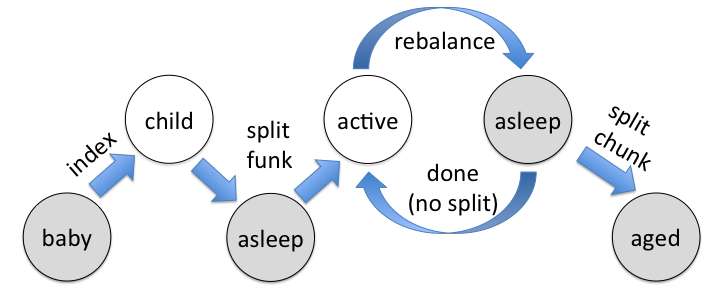
\includegraphics[width=\columnwidth]{state-diagram.png}
}
\caption{Chunk lifecycle; immutable states are grey and mutable ones are white.
Chunk splits  create new chunks in immutable \emph{baby} status, which changes to the mutable \emph{child} state once they 
are indexed. When the appropriate funks are created, the chunks become \emph{active}. All rebalance operations go through an 
\emph{asleep} state when the chunk is immutable.}
\label{fig:status}
\end{figure}

In the third case, the chunk is asleep when we create two new chunks to replace it. 
If the chunk has a munk, we split the munk (by creating two new munks) and update the appropriate pointers in the new chunks.  
Since creating new funks again involves I/O, we do not wish to keep the new chunks immutable for the duration of this process,
and allow funk creation to proceed in the background while the two new chunks still point to the same old funk. 

After we replace the old chunk in the list with the two new ones, 
the old chunk is still accessible via the chunk index (even though it is no longer in the list). 
The new chunks are therefore created in \emph{baby} status, indicating that they are still immutable. 
Once the new chunks are indexed, the old chunk is \emph{aged}, and the new chunks can become mutable.
At this point, we change their status to \emph{child}, indicating that they are no longer immutable, but share a funk with another chunk,
and so should not be rebalanced. Once the funk split completes, we put the chunks to sleep in order
to complete the funk switch and then change their  status  to active. 
The chunk's life-cycle is depicted in Figure~\ref{fig:status}.



\remove{
\subsection{\sys\ operations}
\label{ssec:ops}

\inred{Consider if we want full pseudocode}
}










\section{Implementation}
\label{sec:impl}
We implement \sys\ in C++. We borrow the \code{SSTable} implementation from the RocksDB open source~\cite{RocksDB}.
Similarly to RocksDB, we use \code{jemalloc} for memory allocation.  

The chunk index is implemented as a sorted array holding the minimal keys of all chunks.  
Whenever a new chunk is created (upon split), the index is rebuilt and the reference to the index is atomically flipped. 
We found this simple implementation to be fastest since splits are infrequent. 

\remove{
\paragraph{Synchronization data structures.}
%We note that 
Using a single pending array to synchronize all
operations can cause unnecessary contention.
We mitigate this problem in our implementation by maintaining two data structures for coordinating different operations (similar to~\cite{kiwi}). The first is a per-chunk pending put array (\emph{PPA}) which 
either indicates the current update's key and version, or indicates that the thread is currently not performing a put.
%maps each thread either to a cell in the chunk that the thread is currently attempting to put into and a corresponding version, or an indication that the thread is currently not performing a put. 
The second is a global pending scan array (\emph{PSA}) which tracks versions used by pending scans for compaction purposes; each entry consists of a version \code{ver} and a sequence number \code{seq}, as well as the scan’s key range. Each entry in the \code{PPA}s and \code{PSA} includes, in addition to the operation metadata, an ABA sequence number. 

A put operation consists of 5 phases: (1) \emph{pre-process} - locate the target chunk; if a munk exists, prepare a cell to insert the value into; (2) \emph{publish} - obtain a version while synchronizing with concurrent scans and rebalances via the chunk's lock and publish indication in the chunk's \code{PPA}; (3) \emph{persist} - write the data into the log, indicate it is persisted in the \code{PPA}; (4) \emph{link} - if a munk exists, connect the new cell to the linked list, so it can be found through the list traversal, otherwise, update the row cache to latest version if key is present in the cache; and finally (5) \emph{clean} - clear the entry in the chunk's \code{PPA}, and increase the entry's ABA number.
If the put fails to acquire the chunk's lock (since it is being rebalanced), the operation restarts, and {\inred{re-attempts to}} find an active chunk.
Puts trigger both munk and funk rebalances. The former are handled inline when the munk {\inred{is close to overflow}}; the latter are done in the background 
by helper threads.

%Thus the version number is composed of the GV and 
A per-chunk linearization counter is used to determine the order of concurrent put operations updating the same key.  
Note that multiple \emph{generations} of munks may exist for a chunk throughout its life time.
Therefore, the linearization counter is composed of three parts: (a) the GV value; (b) a \emph{generation number} - incremented whenever a munk is cached into memory and when the munk is rebalanced; and (c) a \emph{sequence number} - incremented upon each put and set to the number of KV-pairs in a munk upon a new generation number. When a new chunk is created as a result of a split, the children chunks inherit their generation number from their parent. The linearization counter is written both to the \code{PPA} upon publishing the put operation, and to the \code{log} when persisting the data. This ensures all operations see the same order of writes per key.

A scan operation first publishes its intent to obtain a version in the \code{PSA}. It determines its scan time $t$ by increasing GV and writing it to its entry in the \code{PSA}. The scan operation then starts traversing the chunks in its range. For each chunk, it first waits for all put operations that are either with smaller version than $t$ or still have not acquired a version to clear their entry in the \code{PPA} or acquire a larger version. After waiting for all concurrent puts to complete, the scan  can read the range from the chunk. If a munk exists, it simply reads the range from the linked list, skipping versions that are not last before $t$. Otherwise, the scan merges the \code{SSTable} and \code{log} data and reads the range from the result, again skipping the penultimate versions. When the scan completes, it clears the entry in the \code{PSA}, and increases the entry's ABA number. Get operations access neither the \code{PSA} nor the \code{PPA}.% data structures.

A munk rebalance iterates through the \code{PSA} to collect the maximum version number among the active scans that cannot be reclaimed yet. If a scan published its intent in the \code{PSA} but published no version number yet, the rebalance waits until either the version is published or the ABA number in the entry is increased. 
\remove{It then acquires the chunk's lock to block additional put operation. If executing a funk rebalance it also acquires the funk rebalance lock for the chunk. After completing the rebalance operation and placing the new content of the chunk in place including the updated metadata, all locks are promoted.
}
}

%\paragraph{Adaptive mechanisms.} \sys\ applies two dynamic mechanisms that adapt to the workload. 
The munk cache applies simple LFU eviction policy. %in which the score is a weighted average of the number of accesses per operation type. 
We use exponential decay to maintain the recent access counts, similar to~\cite{tinyLFU}: periodically, all counters are 
sliced by a factor of two. 
The row cache implements a coarse-grained LRU policy using a fixed-size queue of hash tables. 
New entries are inserted into the head table. Once it overflows, a new empty table is added to the head,
and the tail is discarded. Consequently, lookups for recently cached keys are usually served by the head 
table, and unpopular keys are removed from the cache in a bulk, once the tail table is dropped.

The row cache must never serve stale values. %, yet need not contain each and every updated key. 
Therefore, a put updates the cache  if a previous version of that key is already in the cache. 
If the key is not present in the cache, the put does not update it, to avoid overpopulating the cache 
in write-dominated workloads. After a get, the up-to-date KV-pair is added to the head table unless it is already there.
If the key's value already also exists in another table, it is shared by the two versions, to avoid duplication.

\remove{
\paragraph{Chunk merges support.}
%\inred{move to conclusion and future work?}
Our current implementation does not support chunk merges (to defragment the store after massive data deletion). This could be done as 
part of the rebalance procedure (see~\cite{kiwi}).
In \sys\ this entails merging the funks of two chunks. As in the split operation, the rebalance first acquires the  rebalance locks of the chunks to be merged---to ensure exclusiveness. The content of the chunks is merged and written into a new chunk. Finally, the rebalance acquires the chunks' locks for the short period in which the content that was added to the chunks during the merge is written to the log of the new chunk, and the new chunk swaps the old chunks in the list.
}

\section{Evaluation}
\label{sec:eval}
The baseline for our evaluation is RocksDB -- a mature and widely-used industrial KV-store. 
\remove{RocksDB is used as storage layer of multiple popular SQL and NoSQL databases, e.g., MyRocks~\cite{MyRocks} (incarnation of MySQL) 
and MongoRocks~\cite{MongoRocks} (incarnation of MongoDB). RocksDB is an LSM-tree that is highly optimized for both read and write scenarios. 
For example, its compaction scheduling policies are highly tuned to minimize impact on mainstream data access.} 
We use the most recent RocksDB release 5.17.2, available Oct 24, 2018.  
It is worth noting that RocksDB's performance has significantly improved  over the last two years, primarily through 
optimized LSM compaction algorithms~\cite{CallaghanCompaction}.   We also compare against PebblesDB, 
a research LSM tree prototype that reduces  write amplification  and demonstrated performance advantages
over RocksDB in some scenarios~\cite{PebblesDB}. We further attempted to experiment with TokuDB~\cite{TokuDB} -- 
the only publicly available KV-store whose design is inspired by B$^\epsilon$-trees. However, TokuDB crashed 
in all executions with more than one thread, and in all single-threaded executions its performance was 
inferior to \sys's, hence these results are not presented.

% hardcoded subsections symbol since didn't have time to hack cref...
The experiment setup is described in~\S\ref{ssec:setup}. 
Performance results for \sys\ and RocksDB are presented in~\S\ref{ssec:synthetic} (synthetic data) 
and~\S\ref{ssec:prod} (production data). We study  \sys's scalability and sensitivity to  
configuration settings in~\S\ref{ssec:drill}. Finally,~\S\ref{ssec:pebbles} compares \sys\ with PebblesDB.
%\cref{ssec:recover} evaluates its recovery mechanism. 
 
\subsection{Setup}
\label{ssec:setup} 

\paragraph{Testbed.} We employ a C++ implementation~\cite{Cpp-YCSB} of YCSB~\cite{YCSB}, the  de facto standard  
benchmarking platform for KV-stores. YCSB provides a set of APIs and a synthetic workload suite inspired 
by real-life applications. \inred{In order to exercise production workloads, we extend YCSB to replay log files.}
 
% Most modern KV-stores implement  YCSB adapter API's. 
%The platform decouples data access from workload generation, 
%thereby providing common ground for backend comparison. 

A typical YCSB experiment stress-tests the backend KV-store through a pool of concurrent worker threads that drive identical
(synthetic or real) workloads. A synthetic workload is defined by  (1) the ratios of get, put, and scan accesses, and 
(2) a distribution of key access frequencies. 

Our hardware is a 12-core Intel Xeon 5 machine with 4TB SSD disk. Unless otherwise stated, the YCSB driver  
exercises 12 workers. In order to guarantee fair memory allocation across KV-stores, 
we run each experiment within a Linux container with 16GB RAM. 

\paragraph{Metrics.} Our primary performance metrics are \emph{throughput} 
and \emph{latency percentiles}, as produced by YCSB. 
In addition, we measure \emph{write amplification}, namely, bytes written to storage over bytes passed from the application. 
%In order to explain the results, we also explore \emph{read amplification} (in terms of bytes as well as number of system calls per application read).  
%as well as the number of read \inred{ and write} system calls. 
%The OS performance counters are retrieved from the Linux proc filesystem. 

\paragraph{Methodology.} 
%To make sure that the results  are reproduced, 
We run 5 experiments for each data point and present the median measurement. Since experiments are long, the results vary 
little across runs. In all of our experiments, the STD was within $6.1\%$ of the mean, and in most of them below $3\%$. 
%To avoid cluttering the plots, we do not present the STD. 


\paragraph{Configuration.} 
\inred{
All experiments in~\S\ref{ssec:synthetic}, \S\ref{ssec:prod} and~\S\ref{ssec:pebbles} use the default \sys, RocksDB, 
and PebblesDB configurations, to avoid over-tuning. RocksDB's configuration the same as exercised by the public 
performance benchmarks~\cite{RocksDBPerf}. \S\ref{ssec:drill} explores different \sys\/ configurations and provides 
insights on parameter choices. We also follow the RocksDB performance guide~\cite{RocksDBMemoryTuning} to tune 
its memory resources; the results do not affect our conclusions significantly.  Finally, the PebblesDB code includes a fix 
to  a data race reported in the project's repository~\cite{pebbles-git-issue}. }

\sys's default configuration 
allocates 8GB to munks and 4GB to the row cache,
so together they consume 12GB out of the 16GB container. 
The row cache consists of three hash tables.  
The Bloom filters for funks are partitioned 16-way.  
We set the \sys\/ maximum chunk size limit to 10MB, and the rebalance size trigger to 7MB. 
The funk log size limit is 2MB for munk-less chunks, and 20MB for chunks with munks. 
Finally, we focus on the asynchronous logging mode (with synchronous logging the system
is approximately 10x slower, trivializing the results of scenarios that include puts). 
% \inred{for write intensive workloads, and 512KB for other workloads.}

\subsection{Synthetic benchmarks}
%\subsection{\sys\ versus \ RocksDB}
\label{ssec:synthetic} 

\begin{figure*}[tb]
\centering
\begin{subfigure}{0.33\linewidth}
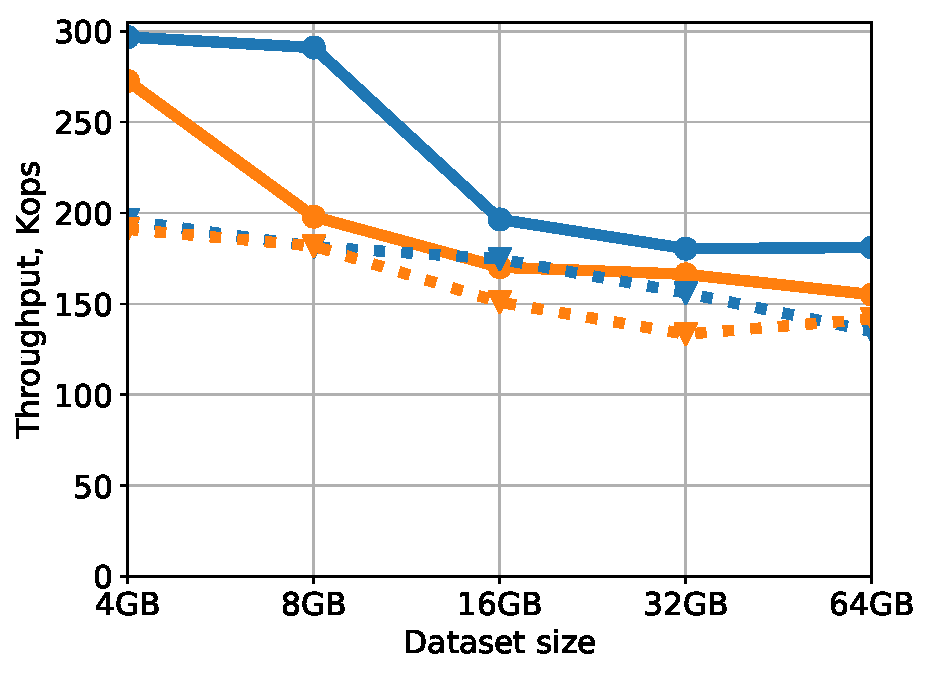
\includegraphics[width=\textwidth]{figs/Workload_P_line.pdf}
\caption{P -- 100\% put}
\label{fig:throughput:p}
\end{subfigure}
\begin{subfigure}{0.33\linewidth}
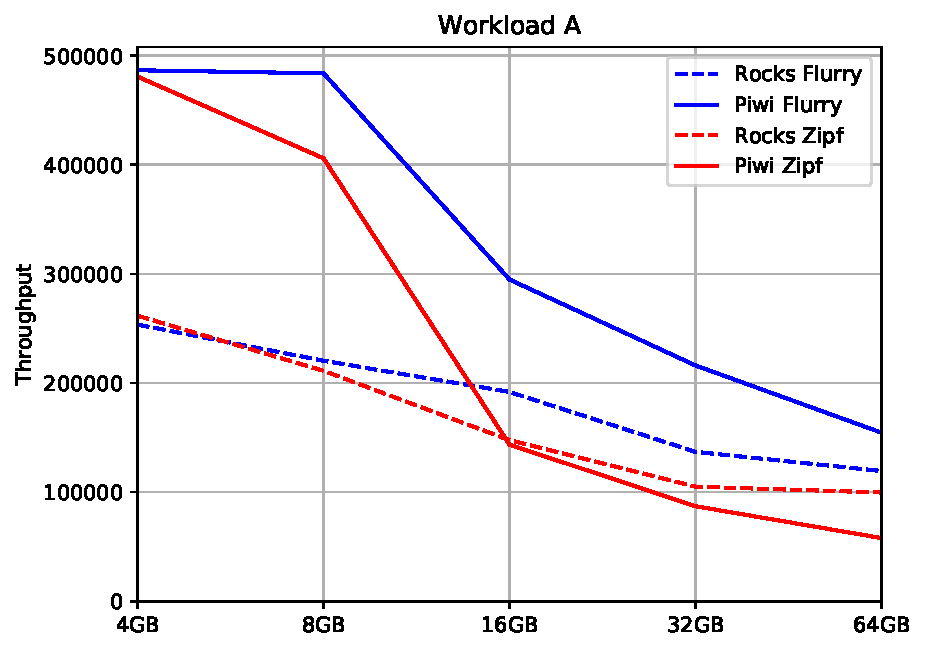
\includegraphics[width=\textwidth]{figs/Workload_A_line.pdf}
\caption{A -- 50\% put, 50\% get}
\label{fig:throughput:a}
\end{subfigure}
\begin{subfigure}{0.33\linewidth}
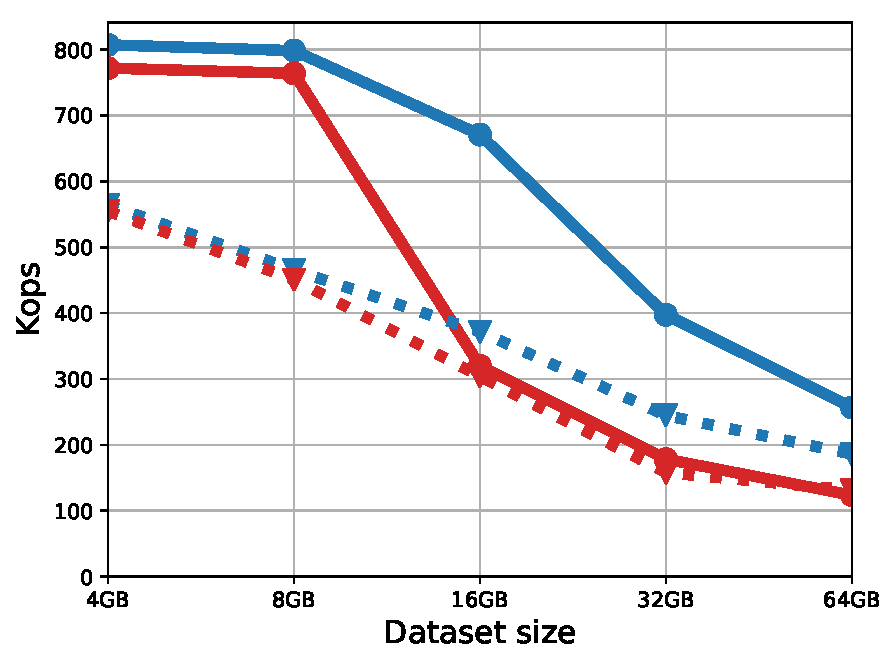
\includegraphics[width=\textwidth]{figs/Workload_B_line.pdf}
\caption{B -- 5\% put, 95\% get}
\label{fig:throughput:b}
\end{subfigure}
\hspace{70pt}
\begin{subfigure}{0.33\linewidth}
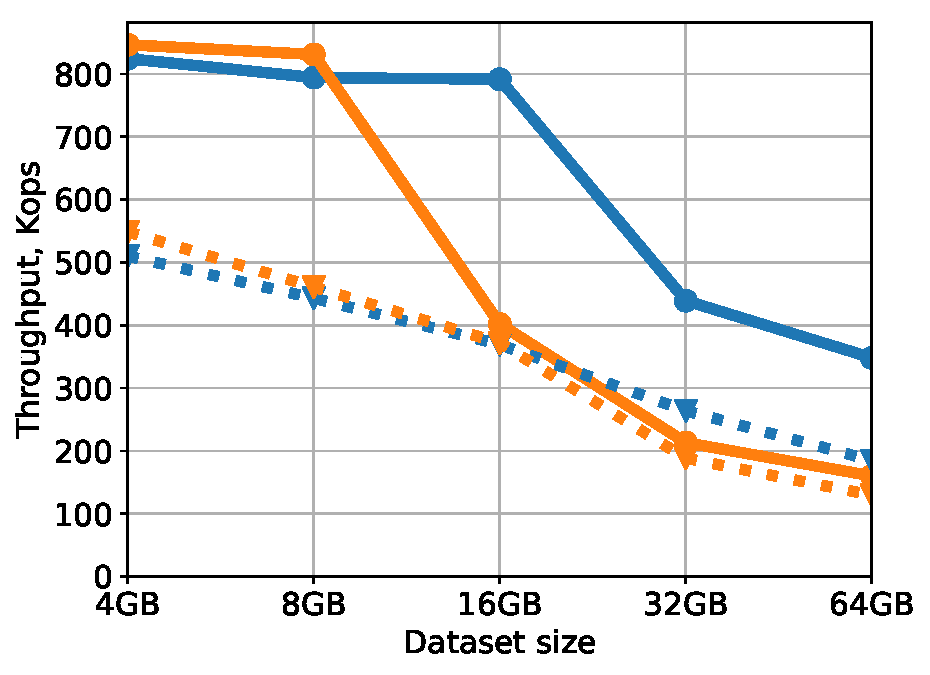
\includegraphics[width=\textwidth]{figs/Workload_C_line.pdf}
\caption{C -- 100\% get}
\label{fig:throughput:c}
\end{subfigure}
\begin{subfigure}{0.33\linewidth}
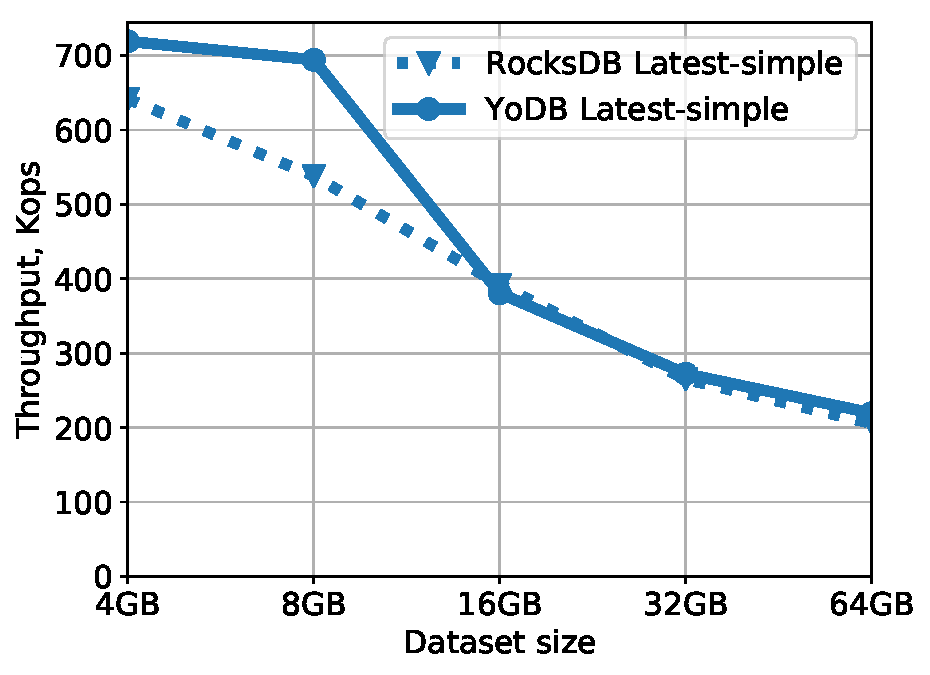
\includegraphics[width=\textwidth]{figs/Workload_D_line.pdf}
\caption{D -- Latest-simple, 5\% put, 95\% get}
\label{fig:throughput:d}
\end{subfigure}
\begin{subfigure}{0.33\linewidth}
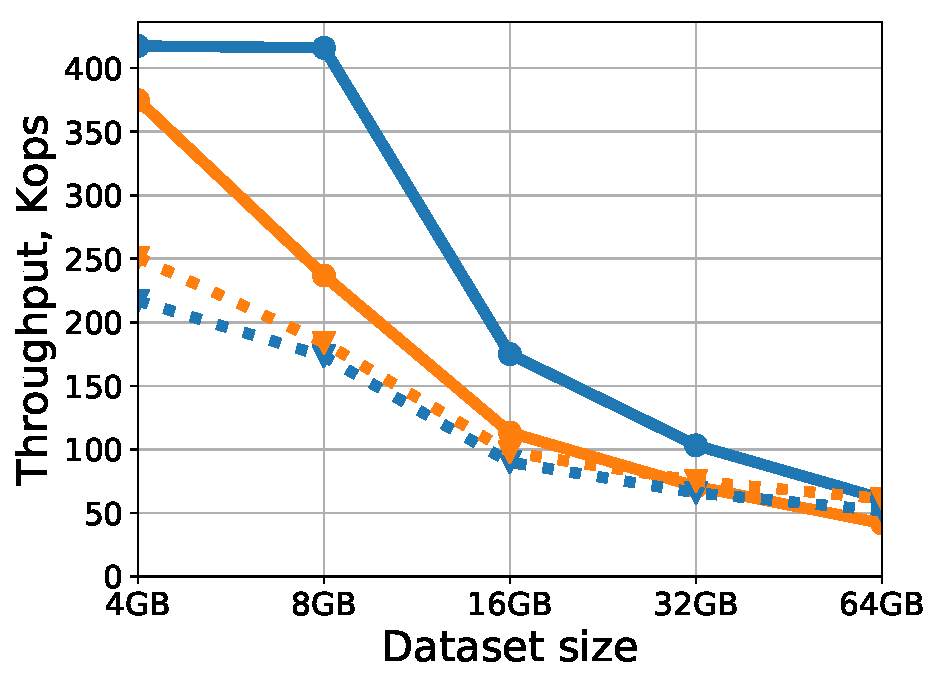
\includegraphics[width=\textwidth]{figs/Workload_F_line.pdf}
\caption{F -- 100\% get-modify-put}
\label{fig:throughput:f}
\end{subfigure}
\hspace{70pt}
\begin{subfigure}{0.33\linewidth}
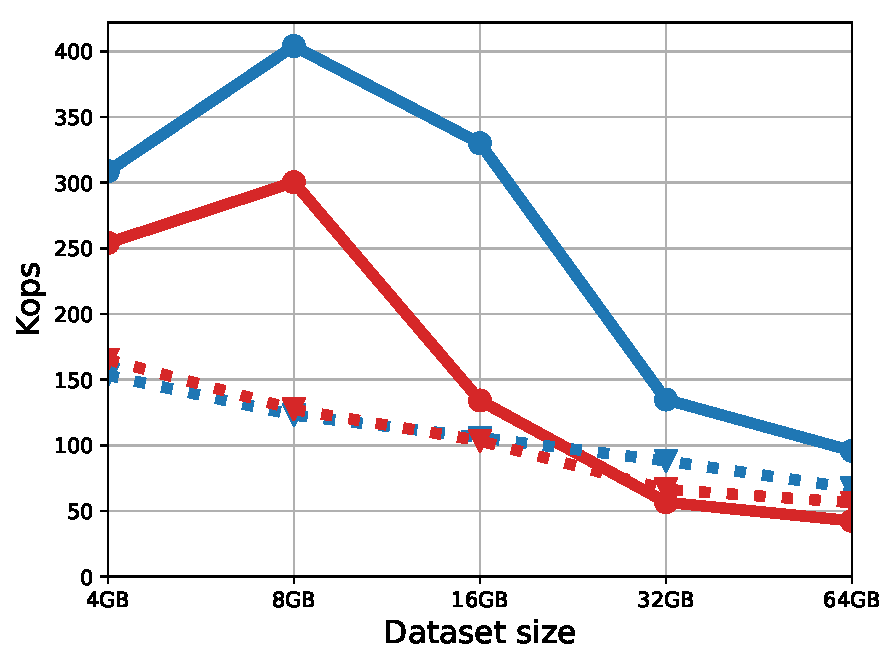
\includegraphics[width=\textwidth]{figs/Workload_E-_line.pdf}
\caption{E10 \\ 5\% put, 95\% scan (10 rows)}
\label{fig:throughput:e10}
\end{subfigure}
\begin{subfigure}{0.33\linewidth}
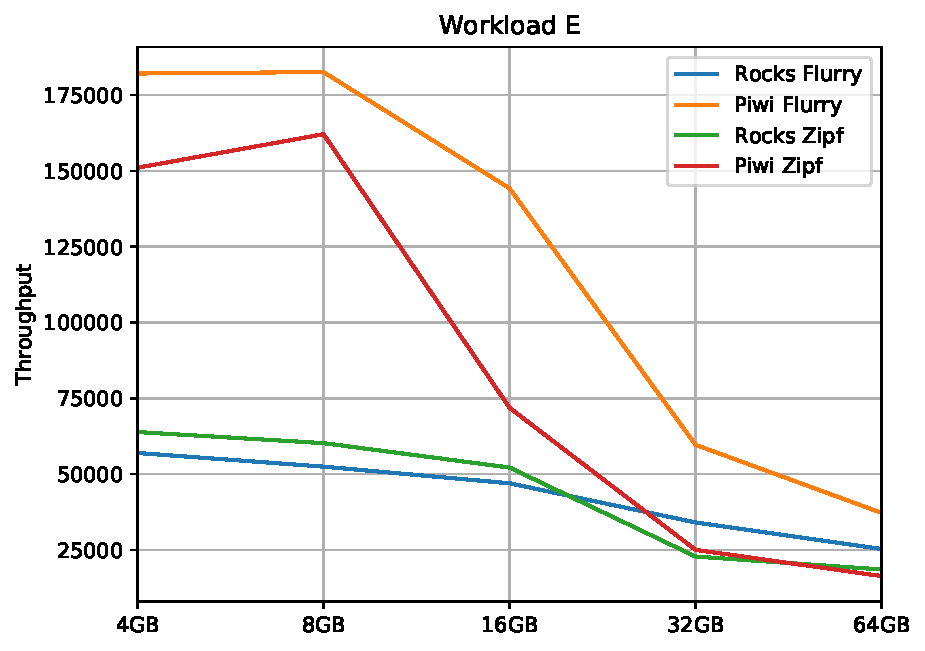
\includegraphics[width=\textwidth]{figs/Workload_E_line.pdf}
\caption{E100 \\ 5\% put, 95\% scan (100 rows)}
\label{fig:throughput:e100}
\end{subfigure}
\begin{subfigure}{0.33\linewidth}
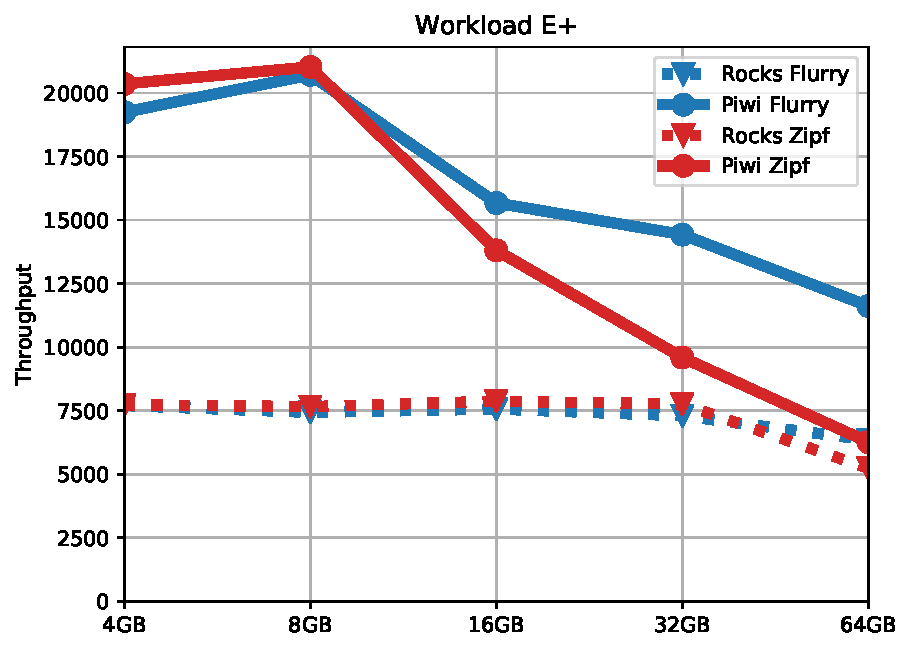
\includegraphics[width=\textwidth]{figs/Workload_E+_line.pdf}
\caption{E1000 \\5\% put, 95\% scan (1000 rows)}
\label{fig:throughput:e1000}
\end{subfigure}
\begin{subfigure}{\linewidth}
\centerline{

\includegraphics[width=0.9\textwidth]{figs/legend.pdf}
\vspace{-5mm}
}
\end{subfigure}
\caption{
{\sys\/ vs RocksDB throughput (Kops), under YCSB workloads with various key distributions.}
}
\label{fig:throughput}
\end{figure*}

We vary the dataset size from 4GB to 64GB in order to exercise multiple locality 
scenarios with respect to the available 16GB of RAM. Similarly to the published RocksDB benchmarks~\cite{RocksDBPerf}, 
the keys are 32-bit integers encoded in decimal form (10 bytes), which YCSB pads with a fixed 4-byte prefix (so effectively, 
the keys are 14 byte long). The values are 800-byte long. The data is stored uncompressed. 


Each experiment consists of three stages. The first stage populates the dataset by filling an initially empty store 
with a sequence of KV-pairs, ordered by key. 
The second phase is warm-up, running read-only operations to warm the caches. The third
phase exercises the specific scenario; all worker threads follow the same access pattern. We 
measure performance only during the steady state (skipping the load and warm-up phases). 
Most experiments  perform 80 million data accesses. Experiments with scans perform 4 to 16 million 
accesses, depending on the scan size. 

\subsubsection{Workloads}
%\paragraph{Workloads.} 


We study the following key-access distributions:  

%\begin{description}
%\item [Zipf-simple] 
\paragraph{Zipf-simple} -- the standard YCSB Zipfian distribution over simple (non-composite) keys. 
Key access frequencies are sampled from the heavy-tailed Zipf distribution 
following the description in~\cite{Gray:1994:QGB:191839.191886}, with $\theta = 0.8$. 
The ranking is over a random permutation of the entire key range, so popular keys are uniformly dispersed.
% The key locations are sampled uniformly at random from the whole data range. 
This workload exhibits medium temporal locality (e.g., the most popular key's frequency is approximately $0.7\%$)
and no spatial locality. 
%This is a standard YCSB workload that captures a multitude of use cases  -- e.g., a web page cache distribution by URL. 

%\item [Zipf-composite]  
\paragraph{Zipf-composite} -- a Zipfian distribution over composite keys. 
The key's $14$ most significant bits comprise the primary attribute. 
The primary attribute is drawn from a Zipf ($\theta=0.8$) distribution over its range. The remainder of the key is drawn uniformally at random.
We also experimented with a Zipfian distribution of the key's suffix; 
the performance trends were similar since performance is most affected by 
 the primary dimension's distribution. Zipf-composite exhibits high spatial locality.% it represents workloads 
%with composite keys.%, such as message threads~\cite{Borthakur:2011:AHG:1989323.1989438},
%social network associations~\cite{Armstrong:2013:LDB:2463676.2465296}, and analytics databases~\cite{flurry},
%and other scenarios with spatial locality of keys, e.g.,  reverse URL domains.

%\item [Latest-simple] 
\paragraph{Latest-simple} -- reading  recently added simple keys (e.g., status updates and reads). 
Keys are inserted in sequential  order; the read keys' distribution is skewed towards recently added ones. 
Specifically, the sampled key's position wrt the most recent key is distributed Zipf. This is a 
standard YCSB workload with medium spatial and temporal locality.

%\item [Uniform] 
\paragraph{Uniform} -- ingestion of keys in random order (the keys are sampled uniformly at random). RocksDB
reports a similar benchmark~\cite{rocksdb-benchmarks}; we present it for completeness.
%\end{description}

The workloads exercise different mixes of puts, gets, and scans. We use standard YCSB scenarios 
(A to F) that range from write-heavy ($50\%$ puts) to read-heavy ($95\%-100\%$ gets or scans). 
In order to stress the system even more on the write side, we introduce a new workload,  
P, comprised of $100\%$ puts; it captures a massive data ingestion scenario. 
%non-sequential data load scenario (e.g., an ETL from an external data pipeline~\cite{flurry}). 

\subsubsection{Evaluation results}
Figure~\ref{fig:throughput} presents throughput measurements of \sys\/ and RocksDB
in all YCSB workloads. Except workload D, which exercises the Latest-simple pattern
(depicted in green), all benchmarks are run with both  Zipf-simple (orange) 
and Zipf-composite (blue). The P (put-only) workload 
additionally exercises the Uniform access pattern (red). \sys\/ results are depicted with solid
lines, and RocksDB with dotted lines. 

We now discuss the results for the different scenarios.
  
\paragraph{ Put-only (data ingestion)} is tested in workload
{P} (100\% put, Figure~\ref{fig:throughput:p}). 
\sys's throughput is 1.8x to 6.4x that of RocksDB's with uniform keys, 1.3x to 2.3x with Zipf-composite keys, 
and 0.9x to 1.6x with Zipf-simple keys. This scenario's bottleneck is the reorganization of persistent data  
(funk rebalances in \sys, compactions in RocksDB), which causes write amplification and hampers performance. 
 
 Under the Zipf-composite workload, \sys\ benefits from spatial locality whereas RocksDB's write performance 
 is relatively insensitive to it, as is typical for LSM stores. For small datasets (4-8GB), \sys\/ accommodates 
all puts in munks, and so funk rebalances are rare. In big datasets, funk rebalances do occur, but mostly in 
munk-less chunks, which are accessed infrequently. This is thanks to \sys\/'s high log size limit for chunks 
with munks. Hence, in both cases, funk rebalances incur less I/O than RocksDB's compactions, 
which do not distinguish between hot and cold data. Note that \sys's recovery time is not impacted by 
long funk logs since they are not replayed upon recovery.

 Under the Zipf-simple workload, the gains are moderate due to the low spatial locality. They are most pronounced 
 for small datasets that fit into RAM.
 
The Uniform workload exhibits no locality of any kind. 
 \sys\/ benefits from this because the keys get dispersed evenly across all chunks, hence all funk logs grow 
 slowly, and funk rebalances are infrequent. The throughput is therefore insensitive to the dataset 
 size. In contrast, RocksDB performs compactions frequently albeit they are not effective (since there are few redundancies). Its throughput 
 degrades  with the data size since when compactions cover more keys they engage more files.
 
 \remove{
 \inred{Increasing RocksDB's block cache size to 5GB is counterproductive in this scenario because it steals 
 resources from the write path (e.g., reducing the throughput by 0.33x for the 64GB dataset under Zipf-simple).}
 }
   
The write amplification in this experiment is summarized in 
Figure~\ref{fig:writeamp}. We see that \sys\/ reduces the disk write rate dramatically, 
with the largest gain observed for big datasets (e.g.,  for the 64GB dataset 
the amplification factors are $1.3$ vs $3.1$ under Zipf-composite, and $1.1$ vs $7.6$ under Uniform). 
%Thus, \sys\/ also reduces disk wear in multiple scenarios. 
%\inred{It should be noted that \sys\/'s low write amplification on the Uniform distribution would have increased on longer runs, as logs fill up and invoke funk rebalances. However, longer runs would have also caused larger RocksDB rebalances.}

%\begin{table}[t]
%\centerline{
%{\small{
%\begin{tabular}{lccccc}
%\hline 
% & 4GB & 8GB & 16GB & 32GB & 64GB \\
%\hline 
%Zipf-composite: &  \multicolumn{5}{c}{}  \\
%RocksDB & 2.08	& 2.29 & 2.35 & 2.40	& {\bf {3.10}}\\
%\sys &  1.33	 & 1.30	& 1.22	& 1.25	& { {\bf 1.34}}\\
%\hline 
%Zipf-simple: &  \multicolumn{5}{c}{}   \\
%RocksDB & 1.92	& 1.95 & 2.02 & 2.20	& 2.44 \\
%\sys &  1.31	 & 1.27	& 1.08	& 1.20	& 1.19 \\
%\hline 
%Uniform: &  \multicolumn{5}{c}{}   \\
%RocksDB & 1.92	& 1.95 & 2.02 & 2.20	& 2.44 \\
%\sys &  1.31	 & 1.27	& 1.08	& 1.20	& 1.19 \\
%\hline 
%\end{tabular}
%}}
%}
%\caption{{\sys\/ versus RocksDB write amplification under the put-only workload P.}}
%\label{fig:writeamp}
%\end{table}

\begin{figure}[t]
	\centering
	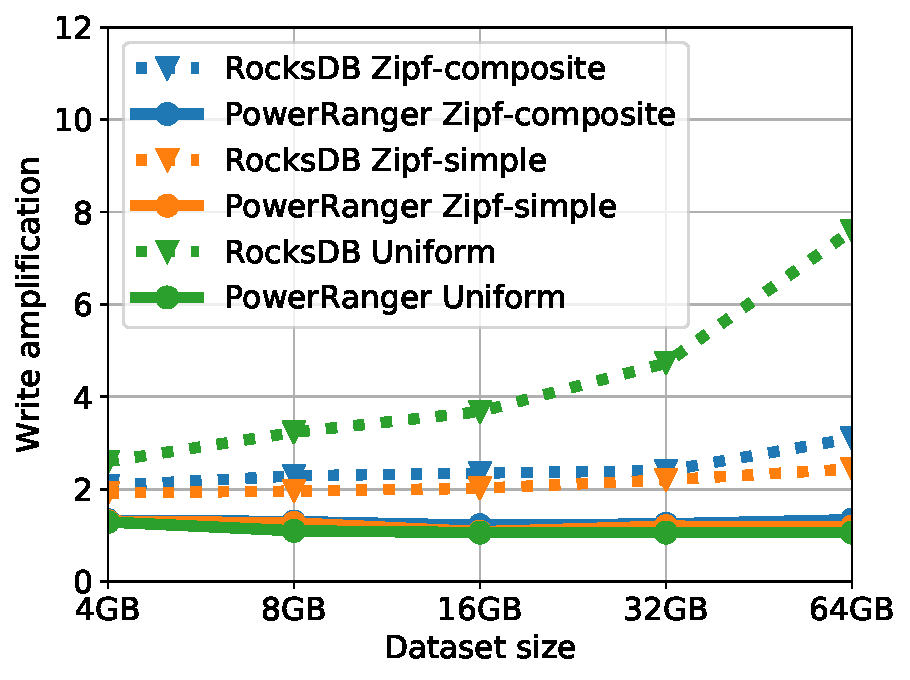
\includegraphics[width=0.35\textwidth]{figs/write_amp_p_line.pdf}
	\caption{{\sys\/ vs RocksDB write amplification under the put-only workload P.}}
	\label{fig:writeamp}
\end{figure}

\remove{
\inred{
\sys\/ advantages are also evident when puts are uniformly distributed (green lines in Figure~\ref{fig:throughput:p}). Since funk rebalances are local, the distribution of rebalances (dictated by the distribution of puts) has little effect. In RocksDB, however, each L0 SST contains keys covering a wide range of keys, causing L0 to L1 compactions to include a large number of SSTs.
}}

\paragraph{ Mixed put-get} is represented in workloads A (50\% put, 50\% get, Figure~\ref{fig:throughput:a}) and 
F (100\% get-modify-put, Figure~\ref{fig:throughput:f}). Note that the latter exercises the usual get and put API (i.e., does not provide atomicity). 
In this scenario, \sys\ works well with composite keys, e.g., in workload A it  achieves $1.4$x to $3.5$x the throughput of RocksDB due to better exploitation of spatial locality. 
With simple keys, on the other hand, the get-put mix is particularly challenging for \sys, which serves many gets from disk due to the
low spatial locality. The bottleneck is the linear search in funk logs, which  fill
up due to the high put rate.
RocksDB's caching is more effective in this scenario, so its disk-access rate in get operations is lower,  resulting in faster gets. 
Note that \sys\/ is still reasonably close to RocksDB in the worst case 
(0.75x and 0.7x throughput for the 64GB dataset in A and F, respectively).
%(In-memory searches are three orders of magnitude faster.)

Figure~\ref{fig:tail_latency}, which depicts tail (95\%) put and get latencies in this scenario, 
corroborates our analysis. \sys\/ has faster puts and faster or similar get tail latencies with composite keys
(Figure~\ref{fig:tail_latency:co}). With simple keys (Figure~\ref{fig:tail_latency:si}),  
the tail put latencies are similar in the two data stores, but the tail get latency of \sys\ 
in large datasets surges.

 To understand this spike, 
we break down the get latency in  Figure~\ref{fig:readstat}. 
Figure~\ref{fig:readstat:dist} classifies gets by the storage  component 
that fulfills the request, and Figure~\ref{fig:readstat:lat} presents the disk search latencies by component. 
We see that with large datasets, disk access dominates the latency.
For example, in the 64GB dataset, $3.3\%$ of gets are served from logs under Zipf-composite, vs $4.0\%$ under Zipf-simple,
and the respective log search latencies are $2.6$ ms vs $4.2$ ms. This is presumably because in the latter, puts are more dispersed, 
hence the funks are cached less effectively by the OS, and the disk becomes a bottleneck due to the higher I/O rate.
%and (2) rebalanced less frequently so their logs grow longer.

\remove{
\begin{figure*}[tb]
\centering
\begin{subfigure}{0.36\linewidth}
\vskip .15in
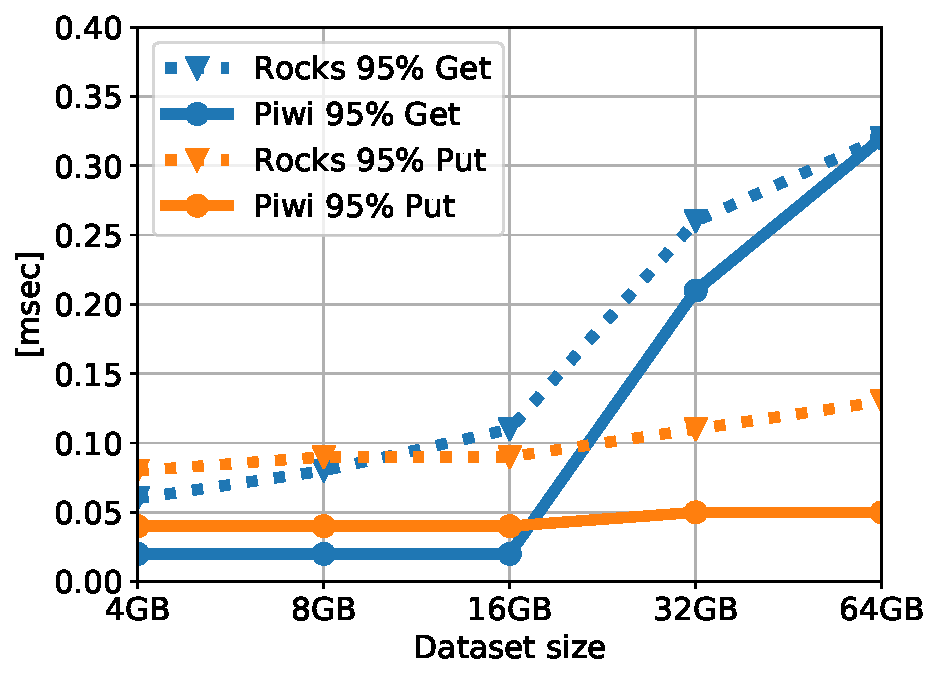
\includegraphics[width=\textwidth]{figs/tail_line.pdf}
\vskip .55in
\caption{95-percentile latency, put and get}
\label{fig:tail_latency:lat}
\end{subfigure}
\begin{subfigure}{0.32\linewidth}
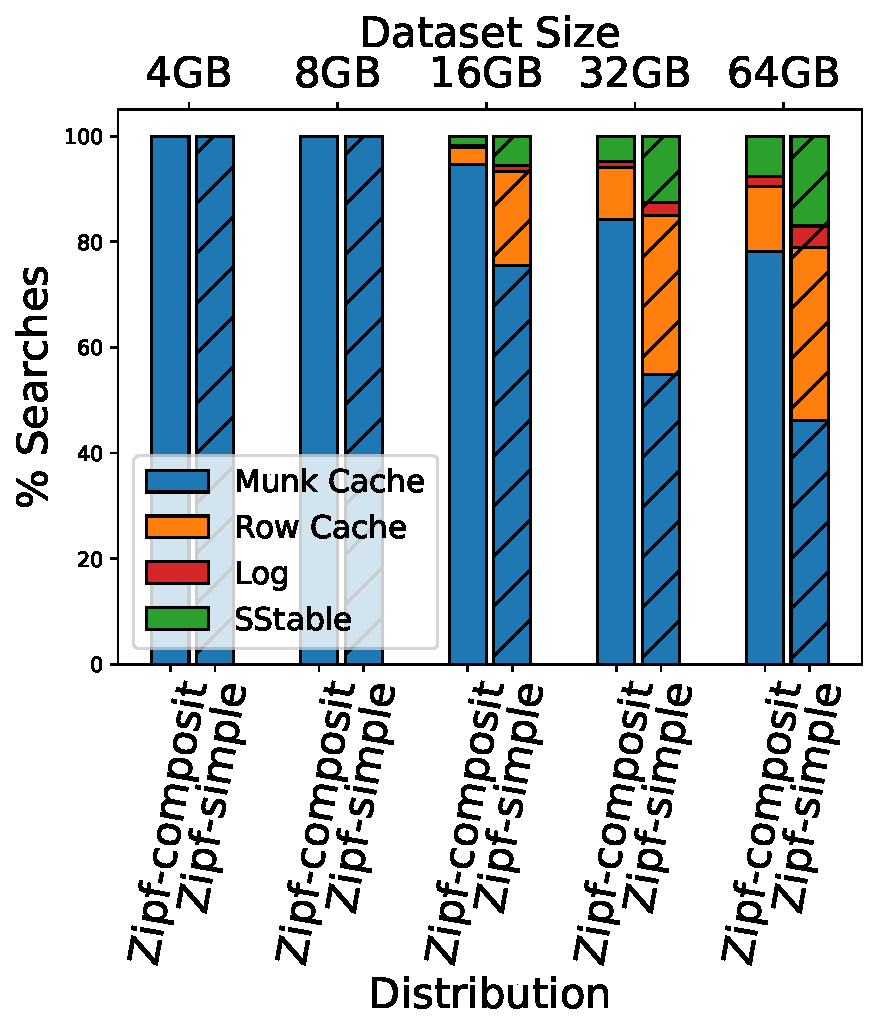
\includegraphics[width=\textwidth]{figs/Time_percentage_A.pdf}
\caption{Fraction of get accesses, by component}
\label{fig:tail_latency:dist}
\end{subfigure}
\begin{subfigure}{0.31\linewidth}
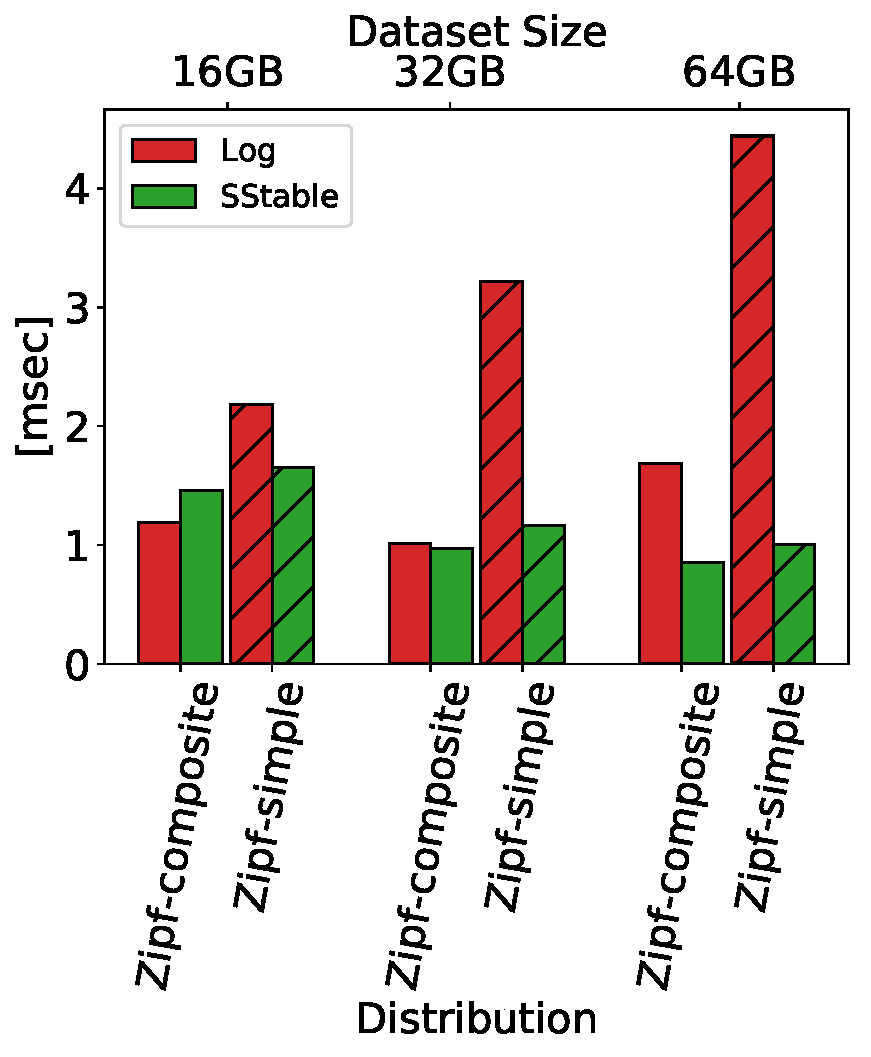
\includegraphics[width=\textwidth]{figs/Latency_A.pdf}
\caption{On-disk get latency, by component}
\label{fig:tail_latency:disk}
\end{subfigure}
\label{fig:tail_latency}
\caption{{\sys\/ tail latency analysis, under a mixed get-put workload A.}}
\end{figure*}
}

\begin{figure}[htb]
\centering
\begin{subfigure}{0.49\linewidth}
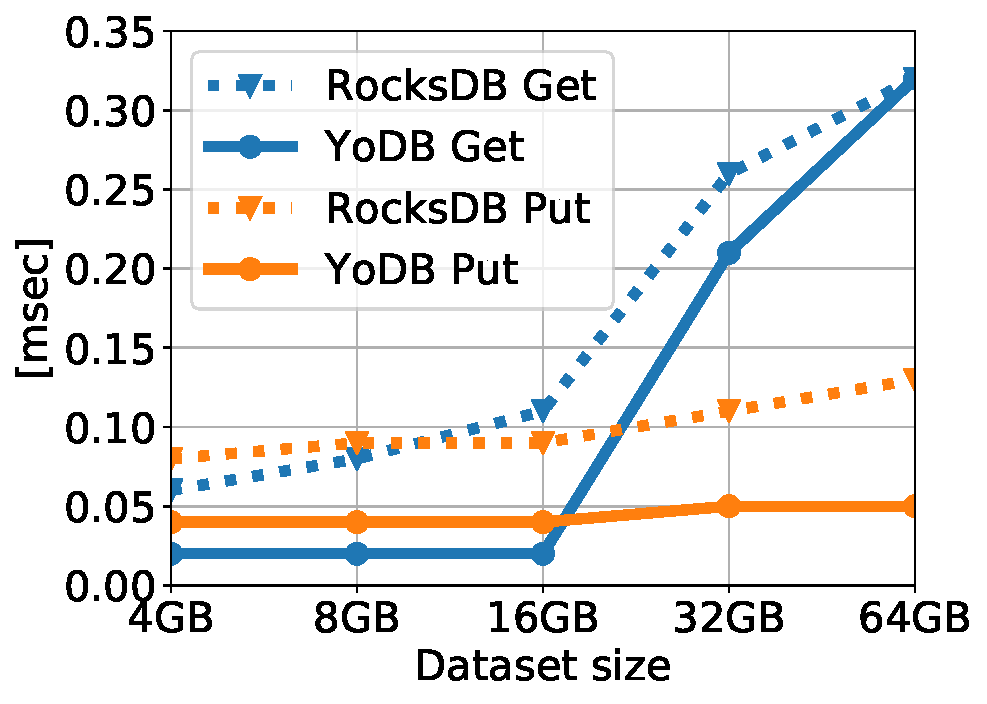
\includegraphics[width=\textwidth]{figs/tail_flurry_line.pdf}
\caption{Zipf-composite}
\label{fig:tail_latency:co}
\end{subfigure}
\begin{subfigure}{0.49\linewidth}
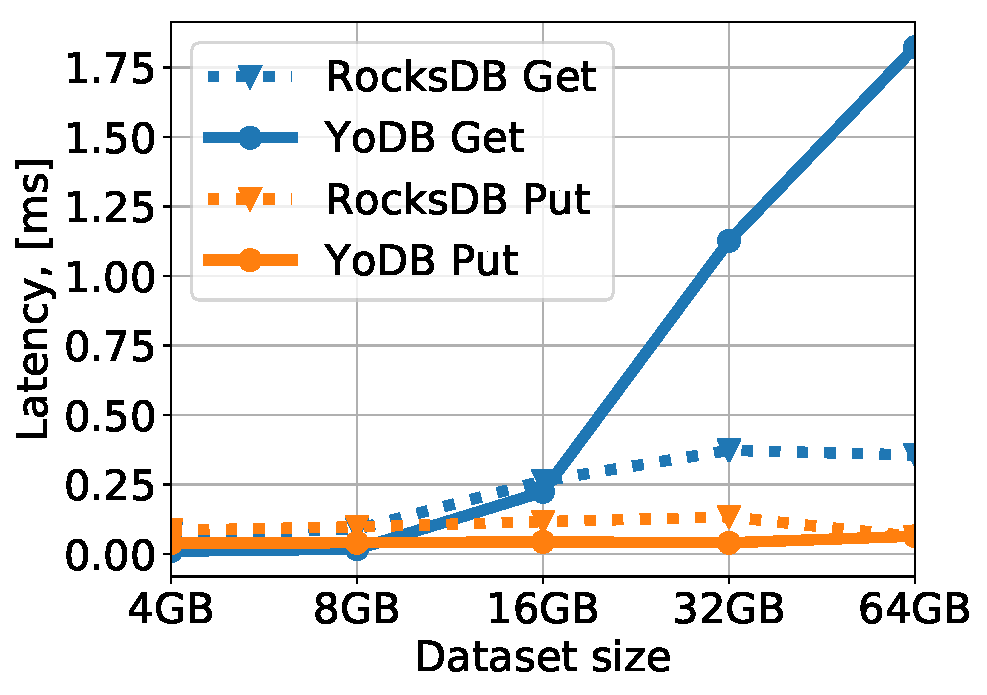
\includegraphics[width=\textwidth]{figs/tail_zipf_line.pdf}
\caption{Zipf-simple}
\label{fig:tail_latency:si}
\end{subfigure}
\caption{{\sys\/ vs RocksDB 95\% latency (ms), under a mixed get-put workload A.}}
\label{fig:tail_latency}
\end{figure}

\begin{figure}[htb]
\centering
%\hspace{0.05\linewidth}
\begin{subfigure}{0.5\linewidth}
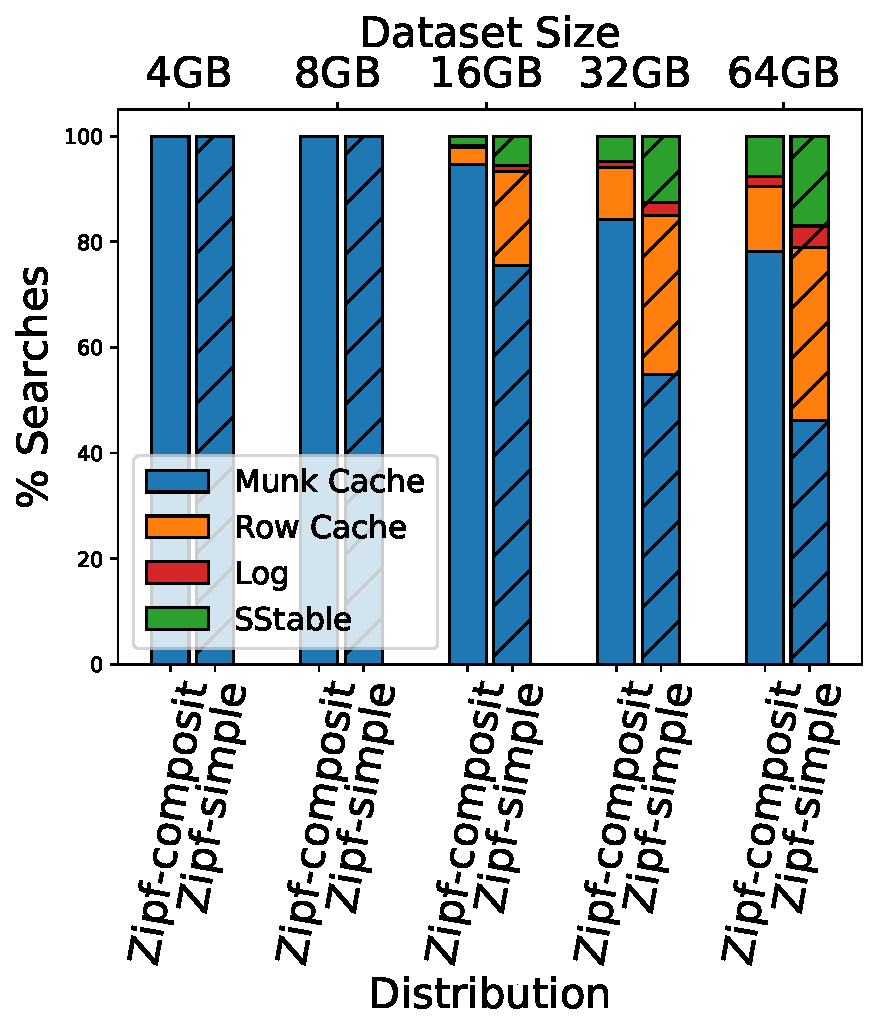
\includegraphics[width=\textwidth]{figs/Time_percentage_A.pdf}
\vskip .1in
\caption{Fraction of get accesses}
\label{fig:readstat:dist}
\end{subfigure}
%\hspace{0.05\linewidth}
\begin{subfigure}{0.49\linewidth}
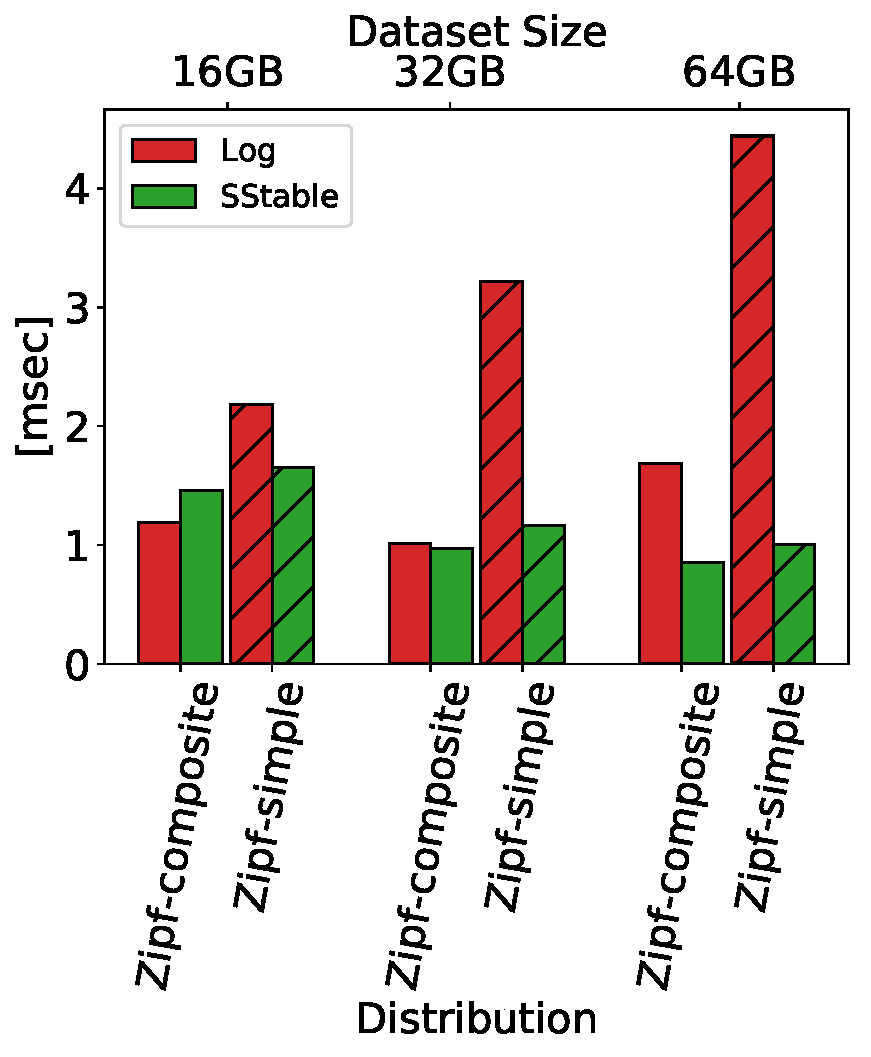
\includegraphics[width=\textwidth]{figs/Latency_A.pdf}
\caption{On-disk get access latency}
\label{fig:readstat:lat}
\end{subfigure}
\caption{{\sys\/ get latency breakdown by serving component, under a mixed get-put workload A.}}
\label{fig:readstat}
\end{figure}

%In-memory caching is paramount. In the same case, the RAM hit rate 
%(munks and row cache combined) is $82.1\%$ with composite keys vs. $79\%$ without them. 
The figure also shows that the row cache becomes instrumental as spatial locality drops -- it serves $32.8\%$ of gets with Zipf-simple 
vs $4.5\%$ with Zipf-composite. 

\paragraph{ Get-dominated} 
workloads (B--D, Figures~\ref{fig:throughput:b}--\ref{fig:throughput:d}) are 
favorable to 
\sys, which has a marked advantage in all key distributions with small datasets (up to the available RAM size) 
and also with Zipf-composite keys in large datasets. 
For example, in workload C (100\% get, Figure~\ref{fig:throughput:c}), 
\sys\/ performs $1.2$x to $2$x better than RocksDB with composite keys,
and up to $1.9$x  with simple ones (for small datasets). 
In these scenarios, \sys\  manages to satisfy most gets from munks, resulting in good performance.
RocksDB relies mostly on the OS cache to serve these requests and so it pays the overhead for invoking system calls. 
As we discuss in~\S\ref{ssec:drill} below, 
RocksDB's performance in this scenario can be improved by using a larger application-level block cache,
but this hurts performance in other benchmarks.

\paragraph{ Scan-dominated} benchmarks (E10--1000,  5\% put, 95\% scan, Figures~\ref{fig:throughput:e10}-~\ref{fig:throughput:e1000})
iterate through a number of items 
sampled uniformly in the range [1,S], where S is  10, 100, or 1000. 
This workload (except with short scans on  large datasets) is favorable to \sys, 
since it exhibits the spatial locality the system has been designed for. 
Under Zipf-composite, \sys\/ achieves $1.4$x to $3.2$x throughput vs RocksDB.   
With simple keys, \sys\ improves over RocksDB when scans are long or the dataset is small. 
In \S\ref{ssec:drill} we show that \sys's scan performance on big datasets can be improved by adapting the 
funk log size limit to this workload. 
%(The experiments reported herein all use the default configuration).
 
\remove{
Note that the scan speed is  higher for the 8GB dataset vs the 4GB dataset. 
Both are quite fast as they are served from memory, but in the smaller dataset there is more contention 
between scans and puts, which slows down   progress. }
%This phenomenon becomes insignificant with longer scans. 

\remove{

\inred{TODO. Zipf-composite reaches 1.2x-2.4x, while zipf-simple starts with 1.5x on 4GB DB, but degrades to 0.7x on 64GB DB. This is the results of an update rate like in A, combined with 100\% read rate. The RMW implementation here was at the YCSB level, hence identical for RocksDB and \sys\/. RocksDB does have a native RMW primitive that works differently (a modification predicate is stored, moving actual computation to gets). \sys\/ doesn't have such a primitive, making the workload less indicative.}

Since workload C only exercises the read path, performance hinges on 
caching efficiency. Both \sys\ and RocksDB benefit from  OS (filesystem) caching in addition to application-level caches. 
Table~\ref{fig:readamp} compares the two systems' read amplification (as a proxy for cache hit ratio) with composite keys, 
in terms of (1) actual disk bytes read and (2) read system calls.  Under the first, 
RocksDB is slightly better in large datasets. However, it relies extensively on the OS cache -- in the 64GB dataset, 
%, at the expense of the user-level block cache. In the same setting, 
it performs almost 12 times as many system calls as \sys,  wasting the CPU resources on  
kernel-to-user data copy. RocksDB developers explain that the block cache scaling potential is limited in their
database, due to tension between its read-path and write-path RAM resources~\cite{RocksDB-default-blockcache-issue}. 
\sys, in contrast, exploits its munk cache for both reads and writes, which leads to better RAM utilization. 


\begin{table}[htb]
{\small{
\begin{tabular}{lccccc}
\hline 
& 4GB & 8GB & 16GB & 32GB & 64GB \\
\hline 
RocksDB, bytes &  0.05 &	0.11 & 0.20 & 0.47 & 0.95\\
\sys, bytes &  0.0 &	0.0 &	0.11	& 0.80	& 1.07 \\
\hline 
RocksDB, syscall & 3.84	& 4.01	& 4.14	& 4.28	& {\bf {4.37}} \\ 
\sys, syscall  & 0.0 & 0.0	& 0.10 & 0.24 & {\bf {0.41}} \\
\hline 
\end{tabular}
}}
\caption{{\sys\/ vs RocksDB read amplification, in terms of bytes and system calls, 
under a read-only workload C with Zipf-composite distribution.}}
\label{fig:readamp}
\end{table}
}


\remove{
\begin{figure}[t]
\centering
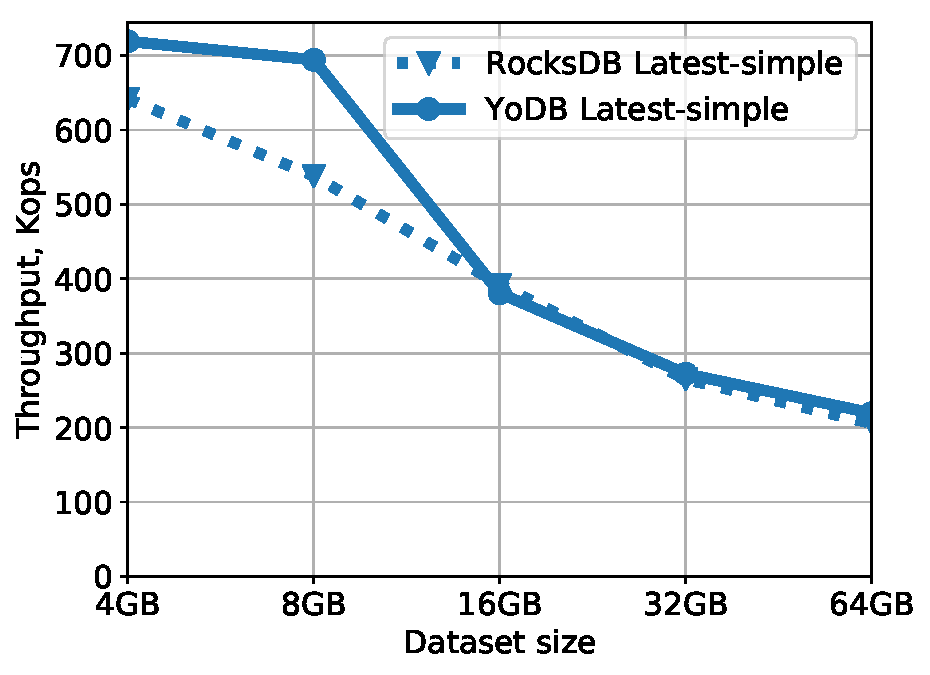
\includegraphics[width=0.4\textwidth]{figs/Workload_D_line.pdf}
\caption{{\sys\/ vs RocksDB throughput, under the D workload.}}
\label{fig:throughput:d}
\end{figure}
}

\subsection{Production benchmarks}
\label{ssec:prod}

\subsection{Insights}
\label{ssec:drill} 

\paragraph{Vertical scalability.} 
Figure~\ref{fig:scalability} illustrates \sys's throughput scaling for the 64GB dataset under Zipf-composite and Zipf-simple  
distributions. We exercise the A, C and P scenarios, with 1 to 12 worker threads.  
As expected, in C (100\% gets) \sys\/ scales nearly perfectly (7.7x for composite keys, 7.8x for simple ones). 
The other workloads scale slower, due to read-write and write-write contention as well as background munk and funk rebalances. 
%P scales 3.8x for both distributions at 8 threads. A scales 6.4x for Zipf-composite and 4.6x for Zipf-simple at 12 threads. 

\begin{figure}[th]
\centering
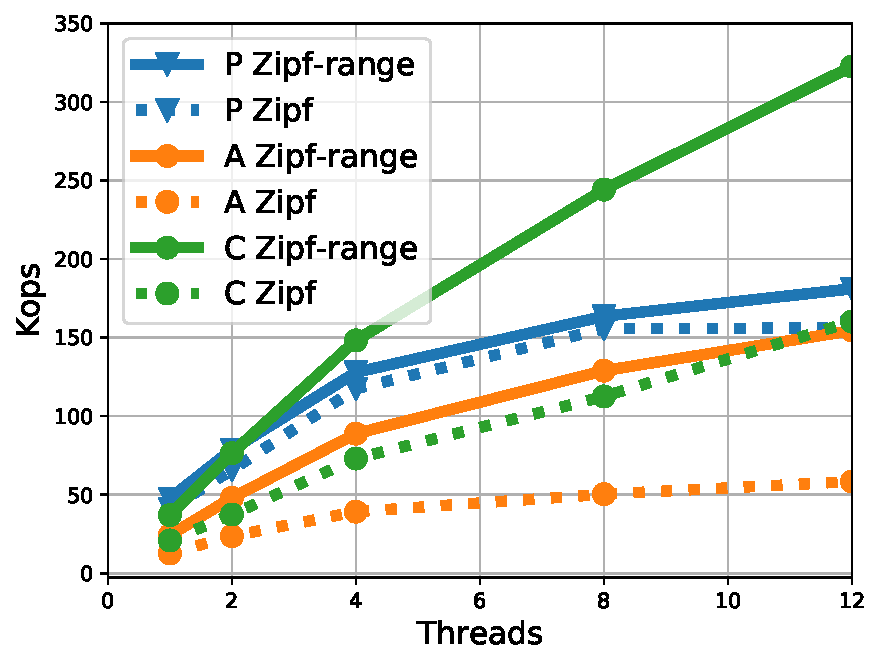
\includegraphics[width=0.4\textwidth]{figs/scalability_line.pdf}

\caption{{\sys\/ scalability with the number of threads for 
the 64GB dataset and different workloads. }}
\label{fig:scalability}
\end{figure}

\remove{
\begin{table*}
\centering
%\begin{subfigure}{0.55\linewidth}
{\small{
\begin{tabular}{l|cccccc|c|ccccc|}
\cline{2-7} \cline{9-13} 
  & \multicolumn{6}{c|}{Maximum log size} & & \multicolumn{5}{c|}{Bloom filter split factor}\\
%\cline{2-7} \cline{9-13} 
& 128KB & 256KB & 512KB & 1MB & 2MB & 4MB & &1 & 2 & 4 & 8 & 16 \\
\cline{2-7} \cline{9-13} 
Zipf-composite: & 50.2	& 55.5 & 80.7	& 134.1 & {\bf {157.5}} & 149.5 & & 134.7 & 133.5 & 140.1 & 152.5 & {\bf {157.4}}   \\
Zipf-simple:    & 27.8	& 30.9 & 36.1	& 58.3  & {\bf {68.3}}   & 68.1   & &  36.3 & 39.2   & 46.3  & 56.0  & {\bf {59.9}}\\
%\hline 
%E, Zipf-range & 29.1	& 36.4 & 36.9	& 37.3	& {\inred{30.4}} & 	37.1 \\
%E, Zipf & 16.1 & 16.3 &	15.8	& 15.8 &	16.4 &	15.8 \\
\cline{2-7} \cline{9-13} 
\end{tabular}
}}
%\caption{Throughput (Kops) vs log size}
%\label{fig:wal:sz}
%\end{subfigure}
%\hspace{0.09\linewidth}
%\begin{subfigure}{0.35\linewidth}
%{\small{
%\begin{tabular}{|l|c|c|c|c|}
%\hline 
%1 & 2 & 4 & 8 & 16\\
%\hline 
%134.7 & 133.5 & 140.1 & 152.5 & {\bf {157.4}} \\
% 36.3 & 39.2 & 46.3 & 56.0 & {\bf {59.9}} \\
%\hline 
%\end{tabular}
%}}
%\caption{Throughput (Kops) vs Bloom filter split factor}
%\label{fig:wal:bf}
%\end{subfigure}
\caption{{\sys\/ throughput under a mixed get-put workload A, 64GB dataset, and different configuration parameters.}}
\label{fig:wal}
\end{table*}
}

\begin{figure}[htb]
\centering
\begin{subfigure}{0.49\linewidth}
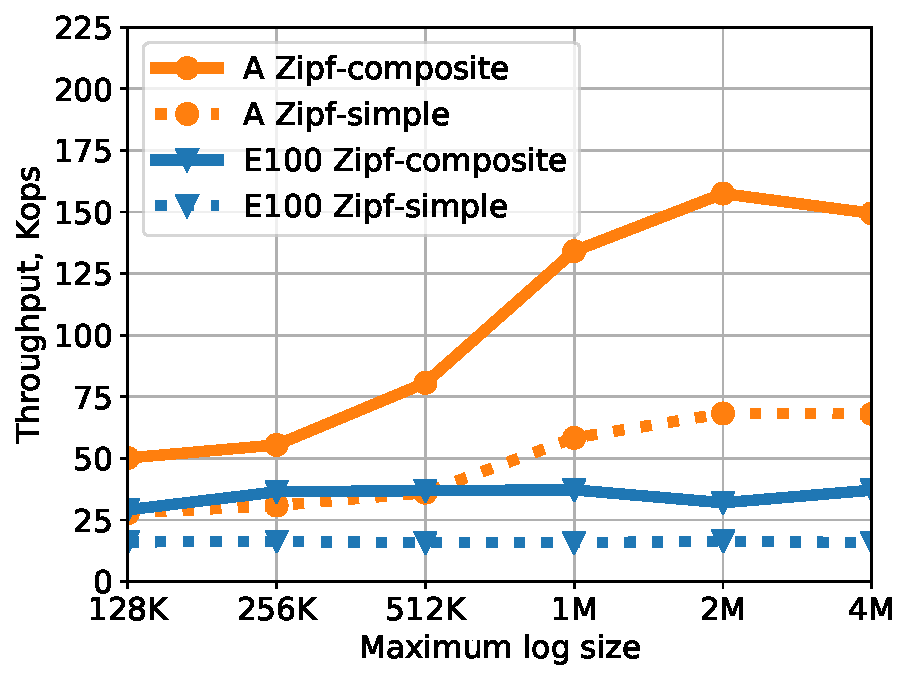
\includegraphics[width=\textwidth]{figs/max_log_size_line.pdf}
\caption{Maximum log size,\\  workloads A and E100}
\label{fig:params:log}
\end{subfigure}
%\hspace{0.05\linewidth}
\begin{subfigure}{0.49\linewidth}
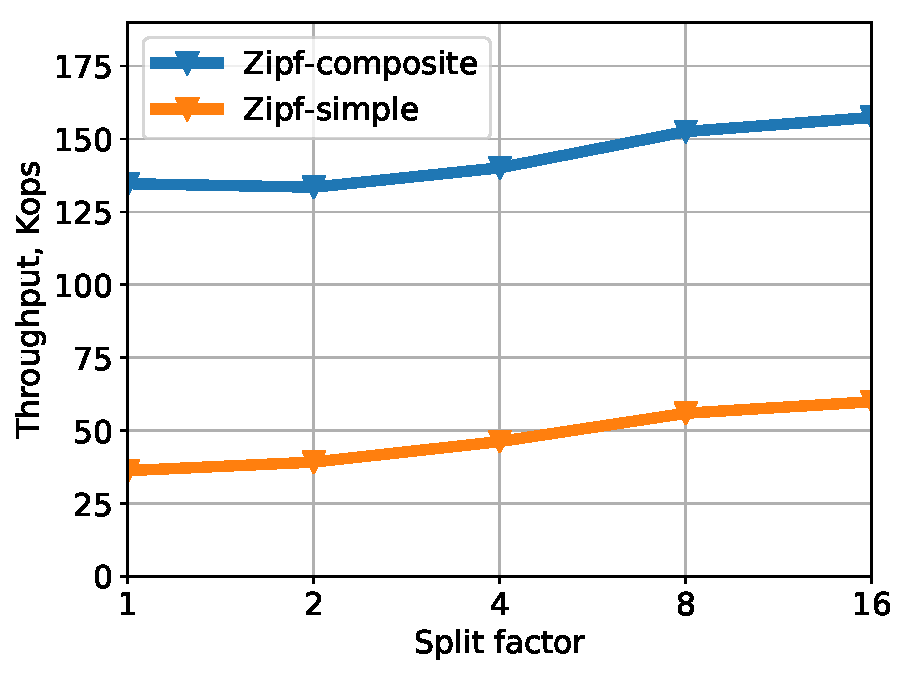
\includegraphics[width=\textwidth]{figs/Bloom_filter_line.pdf}
\caption{Bloom filter split factor,\\ workload A}
\label{fig:params:bf}
\end{subfigure}
\caption{{\sys\/ throughput sensitivity to configuration parameters, on the 64GB dataset under  A (mixed put-get) and 
E100 (scan-dominant, 1 to 100 items).}}
\label{fig:params}
\end{figure}

\paragraph{\sys\/ configuration parameters.} 
We explore the system's  sensitivity to funk-log configuration parameters, for the most challenging 64GB dataset, 
and explain the choice of the default values.

Figure~\ref{fig:params:log} depicts the throughput's dependency on the log size limit of munk-less funks, 
under  A and E100  with the Zipf-composite key distribution. 
The fraction of puts in A is 50\% (vs 5\% in E), which makes it more sensitive to the log size. 
A low threshold (e.g., 128KB) causes frequent funk rebalances, which degrades performance more than 3-fold. 
On the other hand, too high a threshold (4MB) lets the logs grow bigger, and slows down gets. Our experiments  
use 2MB logs, which favors write-intensive workloads. E favors smaller logs, since the write 
rate is low, and more funk rebalances can be accommodated. Its throughput can  grow by up to 20\% 
by tuning the system to use 512KB logs.

Figure~\ref{fig:params:bf} depicts the throughput dependency on the Bloom filter split factor (i.e., the 
number of Bloom filters that summarize separate portions of the funk log) in workload A. 
Partitioning to 16 mini-filters gives the best result; \inred{Idit: the following was not shown: beyond this point the benefit levels off}. 
The impact of Bloom filter partitioning on \sys's %end-to-end get latency as well as the 
memory footprint is negligible.

\paragraph{RocksDB memory tuning.} In RocksDB's out-of-the-box default configuration, the block cache is 8MB. 
We next experiment with block cache sizes of 1GB, 2GB, 5GB, and 8GB. We note that 
RocksDB's performance manual recommends allocating 1/3 of the available RAM 
($\sim$5GB) to the block cache~\cite{RocksDBMemoryTuning}.
The results are mixed. For a small 
dataset (4GB) with composite keys, the block cache effectively replaces 
the OS pagecache, and improves RocksDB's throughput by $1.3$x and 1.6x
for workloads C and E100, respectively, by forgoing the system call overhead. This only partly reduces the gap between
RocksDB and \sys\/ in this setting. 

\begin{figure}[htb]
\inred{Eran please add a graph}
\caption{RocksDB's speedup with larger block caches than its default configuration. Results below $1$ indicate slowdown.}
\label{fig:rocks-memory}
\end{figure}

However, for  bigger datasets (32GB and 64GB),   using a  bigger 
block cache degrades  RocksDB's performance. Figure~\ref{fig:rocks-memory} shows 
RocksDB's speedup with different block cache sizes for the 64GB dataset in the various workloads. 
We see that the default configuration gives the best results for most of the workload suite (i.e., the 
speedups are mostly below $1$). We therefore used this configuration  in~\S\ref{ssec:synthetic} above.   

\subsection{\sys\ versus PebblesDB}
\label{ssec:pebbles} 

We compare \sys\ to PebblesDB, which was shown to significantly improve over RocksDB~\cite{PebblesDB},
mostly in single-thread experiments, before RocksDB's recent version was released.  
We compare \sys\ to PebbelesDB in a challenging  scenario for \sys, with a 32GB dataset and the Zipf-simple key 
distribution. We run each YCSB workload with 1, 2, 4, and 8 threads. The results are summarized in Table~\ref{fig:pebbels-throughput}. 
In all experiments, \sys\ is consistently better than PebblesDB, with its performance improvements ranging from \inred{1.5x} with a single thread
on P, to \inred{4.5x} with eight threads on E10.  In all benchmarks, 
 \sys's advantage grows with the level of parallelism. 
\inred{  
We observed a similar trend with smaller datasets. 
Idit: can we say more?
}

We note that in our experiments, RocksDB also consistently outperforms PebblesDB. 
The gap with the results reported in~\cite{PebblesDB} 
can be attributed, e.g., to RocksDB's evolution, resource constraints (running within a 
container), different hardware, and increased benchmark parallelism.   

\begin{table}
\centering
{\small{
\begin{tabular}{ccccccc}
%Workload & Zipf-simple & Zipf-composite \\
P & A & B & C & D& E10--1000 & F \\
\hline 
1.5--2.9x & \inred{TBD} & \inred{TBD} & 2.1--3.2x &  \inred{TBD} & 2.2--4.5x &  \inred{TBD}  \\
\end{tabular}
}}
\caption{{\sys\/ throughput improvement over PebblesDB, on a 32GB dataset with Zipf-simple keys, with 1 to 8 threads.}}
\label{fig:pebbels-throughput}
\end{table}




  

\section{Related Work}
\label{sec:related}


%common LSM stores RocksDB, scylladb, HyperLevelDB, LevelDB, hbase, cassandra
The vast majority of industrial mainstream NoSQL KV-stores are  implemented as LSM trees~\cite{hbase, 
RocksDB, scylladb, Bigtable2008, cassandra2010}, building on the foundations set by O'Neil 
et al.~\cite{DBLP:journals/acta/ONeilCGO96, Muth1998}. 

Due to LSM's design popularity, much effort has been invested into working around its bottlenecks.
A variety of compaction strategies has been implemented in production systems~\cite{CallaghanCompaction, 
ScyllaCompaction} and research prototypes~\cite{triad, PebblesDB, vttrees, slmdb}. Other suggestions include storage
optimizations~\cite{WiscKey, PebblesDB, vttrees, slmdb}, boost of in-memory parallelism~\cite{scylladb, clsm2015}, and leveraging 
 workload redundancies to defer disk flushes~\cite{triad, accordion}. 

A number of systems focus on reducing write amplification.
PebblesDB~\cite{PebblesDB} introduces fragmented LSM trees in which level files are 
sliced into {\em guards\/} of increasing granularity and organized in a skiplist-like layout. This structure 
reduces write amplification. In contrast, \sys\/ eliminates the concept of levels altogether, 
and employs a flat storage layout instead. WiscKey~\cite{WiscKey} separates key and value storage 
in SSTables, also in order to reduce amplification. This optimization is orthogonal to \sys's concepts,
and could benefit our work as well. 
VT-Trees~\cite{vttrees} are LSM-trees that apply a stitching policy to avoid re-writing already sorted data. This improves performance and significantly reduces write amplification in sequential workloads like time-based ingestion, and file-system workloads. 
SLM-DB~\cite{slmdb} reduces write amplification by having only a single level of SSTable files on disk, supporting a selective compaction policy, and
exploiting persistent memory to eliminate the WAL. To expedite reads, it maintains a B$^+$-tree index that points to KV pairs on disk. Scans benefit from the spatial locality of keys in the B$^+$-tree leaves. Never the less, LSM-like temporal partitioning is used, and the actual values are retrieved from disk.

In-memory compaction was previously employed by
Accordion~\cite{accordion}, which splits the LSM in-memory buffer into mutable 
and immutable levels. Levels are periodically merged and compacted, 
in order to reduce disk flushes. This mechanism is similar to munk rebalance in \sys, 
but the latter rebalances data at the chunk level and so benefits from spatial locality.
%maintains a small dynamic  to absorb write operation. This active component is frequently merged with a larger immutable in-memory component by running at the background. 



\sys's design resembles classic B-trees~\cite{Knuth:1998:ACP:280635} supporting direct random updates to leaf blocks (similar to chunks). 
It resolves the B-tree write throughput limitation \inred{through munks} and in-memory compaction. \inred{TODO: munks don't directly save writes, but they do reduced funk rebalance rate}
% B-trees, which have been designed
%prior to multi-versioning concurrency control (MVCC) methods, heavily rely on locks for consistency of operation; this method is 
%inferior to MVCC in terms of performance.
%heavily rely on exclusive locks for concurrency control~\cite{Lehman81}. \sys\ operations use locks in shared mode in normal flow; exclusive mode is only used by background rebalance operations. }


In  recent years, $B^{\epsilon}$-trees~\cite{Brodal:2003:LBE:644108.644201} have been used in production KV-stores~\cite{TokuDB} and filesystems~\cite{BetrFS}. 
A $B^{\epsilon}$-tree is a B-tree variant that uses overflow buffers in internal nodes.
% trading buffer compactions for random I/O.
Buffering allows writes to be combined, but lookups are slowed down by having to search the unordered buffers.
% \sys\/ applies similar ideas to leaf-level storage. TokuDB's~\cite{TokuDB} performance 
%is on par with RocksDB in many use cases, but its disk image tends to be bigger~\cite{tokudb-vs-rocksdb}.
%We are not aware of any  $B^{\epsilon}$-tree implementation that provides atomic scans and zero-time consistent recovery as \sys\ does. 
%Similarly to \sys, keys and values are appended to buffers, and pointers to keys are sorted in contiguous segments, 
%thereby improving read performance. 
$B^{\epsilon}$-tree and \sys\/ designs are compared in~\cref{sec:design}.

Tucana~\cite{tucana} is a $B^{\epsilon}$-tree optimization that uses three techniques to reduce overheads: copy-on-write, 
private allocation, and memory-mapped I/O.
\inred{ \sys\/ could incorporate some of these to further improve performance. 
However, Tucana paper does not provide consistent semantics for scans that span multiple leaf segments. TODO: replace with some email summary...}

In-memory KV-stores~\cite{ignite, redis, memcached, Srinivasan:2016:AAR:3007263.3007276} have originally emerged as fast volatile 
data storage, e.g., for web and application caches. Over time, many of them evolved to support durability,
%albeit as a second-class citizen in most cases. 
albeit they still require the complete data set to be memory resident.
%For example, Ignite~\cite{ignite} uses a B-tree index with in-place random updates. 
%These systems resemble \sys\/ in their memory-centric approach. 
We are unaware of the consistency guarantees or performance optimizations with respect  to disk-resident data in such systems. 

%Their persistent storage support is based on either B-tree~\cite{ignite} or LSM-tree design~\cite{redis}. 
%used for application data caching, but also as building blocks for distributed database with optional durability~\cite{ignite,redis}. These are not comparable with \sys\ as they are either not persistent~\cite{memcached}, do not support atomic scans~\cite{redis} or resemble  relational DBMS with a centralized WAL, , and in-place updates~\cite{ignite}  more than a KV LSM store.

\section{Conclusions}
\label{sec:conclusions}
We presented \sys\/ -- a novel persistent KV-store optimized for workloads with high spatial locality, as prevalent in modern %data-driven 
applications. \sys\/ provides strong (atomic) consistency guarantees for random updates, random lookups, and range queries. 
\sys\/ outperforms the state-of-the-art RocksDB LSM store  in the  majority of YCSB benchmarks, with both 
standard and spatially-local key distributions, in which it excels in particular. \sys\/ further reduces write amplification to near-optimal under write-intensive 
workloads. Finally, it provides near-instant recovery from failures.
%, in contrast to traditional data stores based on centralized write-ahead logs.

Beyond building a particular system prototype, this paper puts forth a novel KV-store design alternative that emphasizes spatial locality. We hope to see future realizations of this approach with various improvements, through novel ideas or ones borrowed from other existing solutions. 
%It can also benefit from new hardware trends, in particular, non-volatile memory technologies.  

%\bibliographystyle{acm}
 %\bibliography{ref}

\clearpage
{\normalsize \bibliographystyle{acm}
\bibliography{ref}}

%\theendnotes

\end{document}
